\documentclass[../main]{subfiles}
\ifSubfilesClassLoaded{
    \dominitoc
    \tableofcontentsfile
	\pagenumbering{arabic}
    \setcounter{page}{1}
	\setcounter{chapter}{4}
	\addbibresource{../Biblio/biblio.bib}
}{}


\begin{document}
\chapter{Analyse de l'auto-organisation de CxSOM sur des cartes en une dimension}\label{chap:analyse}
\graphicspath{{06-Analyse/figures},{./figures}}
\minitoc

\`A partir de la méthode expérimentale et de représentation du comportement de l'architecture que nous avons présentée précédemment, nous nous concentrons dans ce chapitre sur l'identification des dynamiques et comportements d'apprentissage d'une architecture CxSOM.
Une architecture CxSOM est composée de $N$ cartes connectées entre elles, pouvant prendre ou non une entrée externe $\inpx\m{i}$. L'objectif de l'architecture est d'appendre une représentation des relations entre les modalités $\inpx\m{i}$.
Ces méthodes de représentation nous permettront dans ce chapitre de caractériser l'organisation d'architecture de deux et trois cartes en une dimension selon leur réponse à différentes dispositions d'entrées.
Nous introduirons ensuite un comportement spécifique à CxSOM~: la prédiction d'entrée. Nous montrerons que la relaxation permet de prédire une entrée manquante, conférant à des cartes de Kohonen une capacité de prise de décision. Nous appliquerons cette propriété de prédiction de CxSOM au contrôle d'un drone.


\section{Mécanismes d'auto-organisation dans une architecture de deux cartes}

\subsection{Introduction}

Nous étudions dans cette section les propriétés d'auto-organisation émergeant d'une architecture de deux cartes sur plusieurs modèles d'entrées jouet en faible dimension. 
Ces modèles nous permettent de maitriser les dépendances entre entrées et ainsi de dégager des comportements d'organisation spécifiques à un modèle d'entrées.

\subsection{Méthode expérimentale}

Dans cette section, nous considérons des architectures de deux cartes en une dimension dans lesquelles chaque carte prend une entrée externe. Ce modèle est présenté en figure~\ref{fig:archis}.
Chaque carte a une taille fixée de 500 n\oe{}uds, indexés entre 0 et 1, et possède deux couches de poids $\w_e$ et $\w_c$. Les rayons de voisinage sont fixés à $r_e = 0.2$ et $r_c = 0.02$, sauf si précisé dans l'expérience.
Les connexions sont réciproques~: $M\m{1}$ prend en entrée contextuelle $\bmu\m{2}$ et inversement.

\begin{figure}[t]
	\centering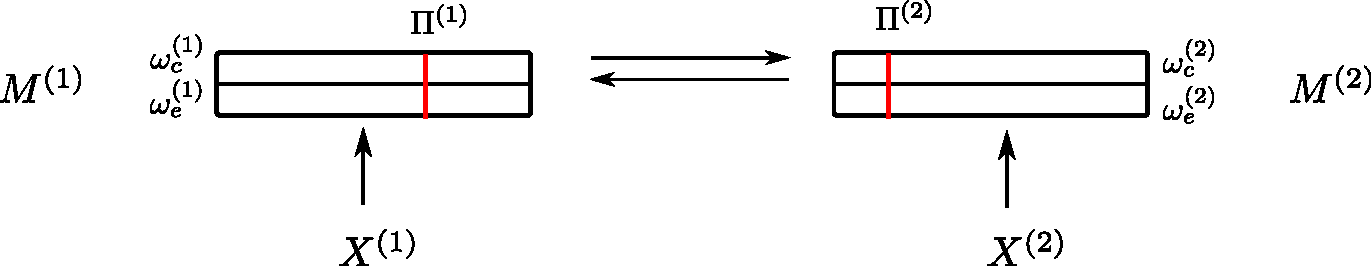
\includegraphics[width=\textwidth]{archi_2maps.pdf}
	\caption{Schéma de l'architecture de deux cartes étudiée et rappel des notations. Chaque carte possède une couche de poids externe et une couche de poids contextuels. Les connexions sont rétroactives~: l'entrée contextuelle de $M\m{1}$ est la position du BMU de la carte $M\m{2}$ et inversement. Chaque carte prend une entrée externe.\label{fig:archis}}
\end{figure}

Rappelons la définition des entrées multimodales~: il s'agit d'un ensemble d'entrées $\mathbf{\inpx} = (\inpx\m{1}, \cdots, \inpx\m{n})$. Nous notons $K$ la dimension totale des entrées.
Nous représentons la dépendance entre entrées en choisissant une variable latente du modèle $U$ telle que :
$$ \forall i, \inpx\m{i} = f\m{i}(U) + \epsilon\m{i}$$
avec $\epsilon\m{i}$ un bruit sur les entrées.
La dimension de $U$ détermine la dépendance entre les entrées.
Une variable $U$ en une dimension paramètre des points placés sur une courbe~; $U$ en 2 dimensions paramètre une surface. Plus généralement, une variable $U$ de dimension $k$ paramètre des entrées de dimension totale $K > k$, positionnées sur une variété de dimension $k$.

Ce modèle est général~: au pire, la dimension de $U$ correspond à la dimension totale des entrées. 
Par ailleurs, de nombreux modèles d'entrées réelles se placent effectivement sur une variété de dimension réduite. Le choix d'un modèle d'entrées géométriques situées sur une variété de dimension inférieure est donc justifié comme modèle expérimental simplifié.

Dans cette série d'expériences, nous étudions un modèle d'entrée de dimension totale $K=2$. Chaque modalité est alors une valeur 1D.
Nous reviendrons d'abord sur le modèle du cercle (\textbf{A}), qui a déjà été présenté au chapitre \ref{chap:repr}. L'intérêt d'utiliser cette courbe est que la disposition est symétrique~: toute entrée $X^{(1)}$ correspond à deux valeurs possibles pour $X^{(2)}$ et inversement. $U$ est une variable 1D.
Nous testerons ensuite si les observations réalisées sur le modèle du cercle se retrouvent pour d'autres dispositions d'entrées, représentées en figure~\ref{fig:input_list}~:
\begin{itemize}
	\item Une entrée est une fonction de l'autre~: $\inpx\m{2} = cos(\inpx\m{1})$~(\textbf{B})
	\item Les entrées sont identiques (cas dégénéré) (\textbf{C})
	\item Entrées sur une courbe de Lissajous (\textbf{D})~: une entrée $\inpx\m{1}$ correspond à 4 à 6 valeurs de $\inpx\m{2}$ et inversement.
	\item Entrées totalement indépendantes, prises aléatoirement dans le carré $[0,1]^2$~(\textbf({E})). $U$ est alors une variable 2D correspondant aux entrées.
	\item Entrées sur un anneau \textbf{(F)}. $U$ est alors une variable 1D avec du bruit dans le modèle d'entrées. Une carte de Kohonen classique a comme propriété d'être résistante au bruit sur les données. Ainsi, une carte 1D se dépliant sur un anneau fin en 2D apprendra d'abord une représentation du cercle sous-jacent. Nous voulons vérifier comment cette propriété se vérifie sur l'apprentissage de données par plusieurs cartes.
\end{itemize}

La génération des entrées suit le processus suivant~: $U$ est tiré uniformément dans $[0,1]$. Le couple d'entrées $(\inpx\m{1},\inpx\m{2})$ généré à partir d'une même valeur de $U$ est présenté à l'architecture lors d'une même itération.
L'apprentissage est réalisé sur un échantillon de 20000 points, générés aléatoirement et présentés une fois. 
Les tests sont réalisés sur 1000 points générés aléatoirement selon la même distribution d'entrées que l'apprentissage.

\begin{figure}[h]
	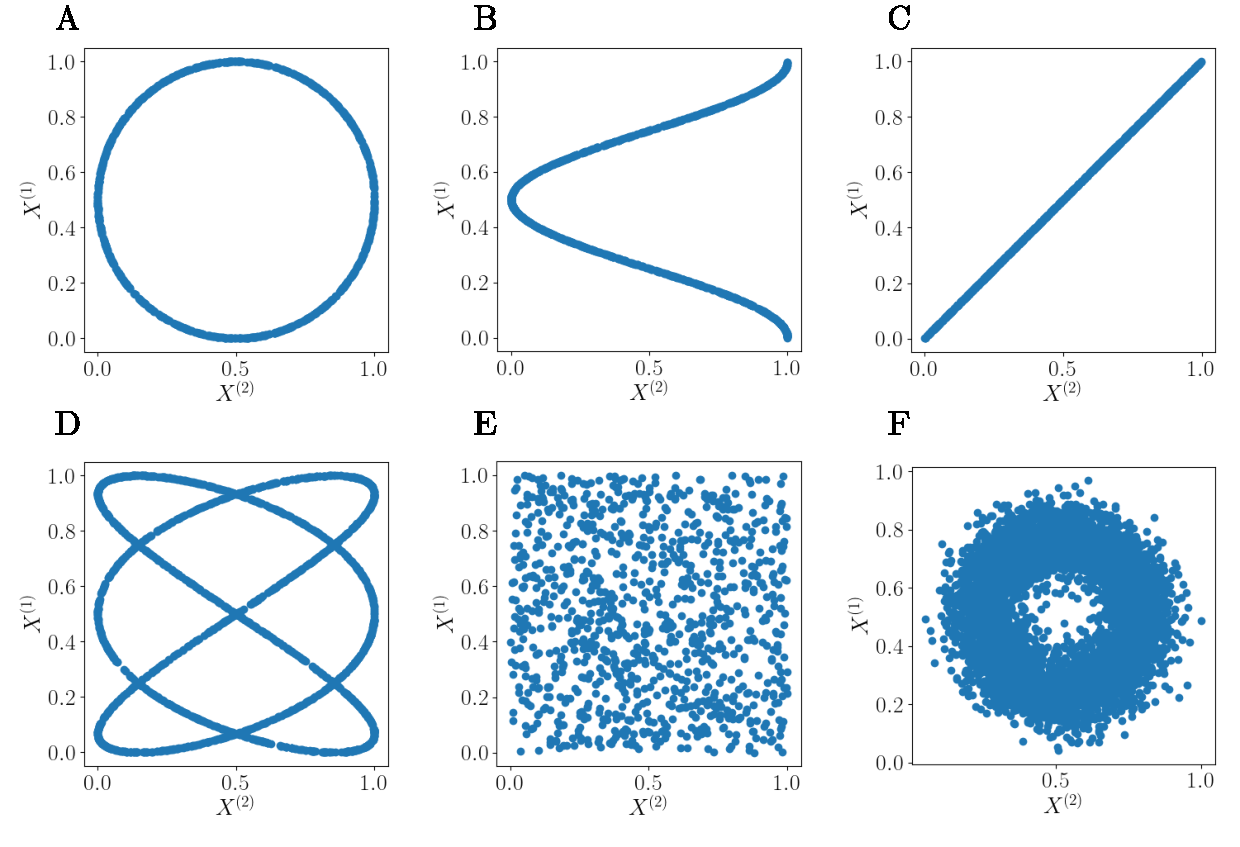
\includegraphics[width=\textwidth]{inputs/inputs.pdf}
	\caption{Dispositions d'entrées en deux dimensions. $M\m{1}$ prend en entrée l'ordonnée $\inpx\m{1}$ et $M\m{2}$ prend en entrée l'abscisse $M\m{2}$. \label{fig:input_list}}
\end{figure}

Le code utilisé pour générer les expériences et les représentations est disponible en ligne \footnote{\url{todo.github.com}}

\subsection{Expérience préliminaire : Entrées disposées en cercle}

Revenons d'abord sur l'expérience précédemment présentée au chapitre \ref{chap:repr}, réalisée sur les entrées disposées selon un cercle (\textbf{A}).
Après avoir vérifié que les poids des cartes convergent bien au cours de l'apprentissage, nous étudierons la disposition finale des poids externes et contextuels.
Nous nous intéresserons enfin à la qualité de représentation de l'entrée externe par les poids externes des BMUs.

\subsubsection{Convergence des poids}

Dans une carte de Kohonen classique, le rayon de voisinage et le taux d'apprentissage sont diminués de façon prédéfinie au cours des itérations. 
Cette opération permet d'assurer un dépliement des cartes au début de l'apprentissage puis assure la convergence des poids $\w$ des cartes lorsque les paramètres sont faibles.
Dans notre étude, nous choisissons au contraire de ne pas modifier les paramètres d'apprentissage au cours des itérations.
Nous vérifions dans cette section la convergence des poids des cartes avant d'étudier l'organisation. 

La figure~\ref{fig:conv} présente l'évolution des variations des poids $\w\ext$ et $\w\cont$ dans chaque carte au cours de l'apprentissage. Toutes les 100 itérations, nous calculons la différence maximale entre $w_t$ et $w_{t-100}$.
Nous observons que cette courbe tend vers $0$ pour chaque courbe de poids. Cela montre que tous les poids de la carte tendent vers une position stable.

Les observations montre qu'une carte se comporte d'abord comme une carte de Kohonen classique apprenant sur des entrées externes, ce qui s'explique par la différence de contribution dans l'activité globale des activations externes et contextuelles, calculée par~: 
$$ a_g = \sqrt{a_e \cdot (\beta a_e + (1-\beta)a_c)}$$
Les entrées contextuelles viennent seulement moduler le calcul de l'activité externe.
Notons toutefois que nous sommes sur un cas particulier de cartes 1D sur des entrées 1D.
La convergence en l'absence de décroissance de paramètres peut poser plus de problèmes sur des cartes en deux dimensions. 
Nous verrons que pour des rayons de voisinage bien choisis, la convergence sera possible également en deux dimensions.

\begin{figure}[h!]
	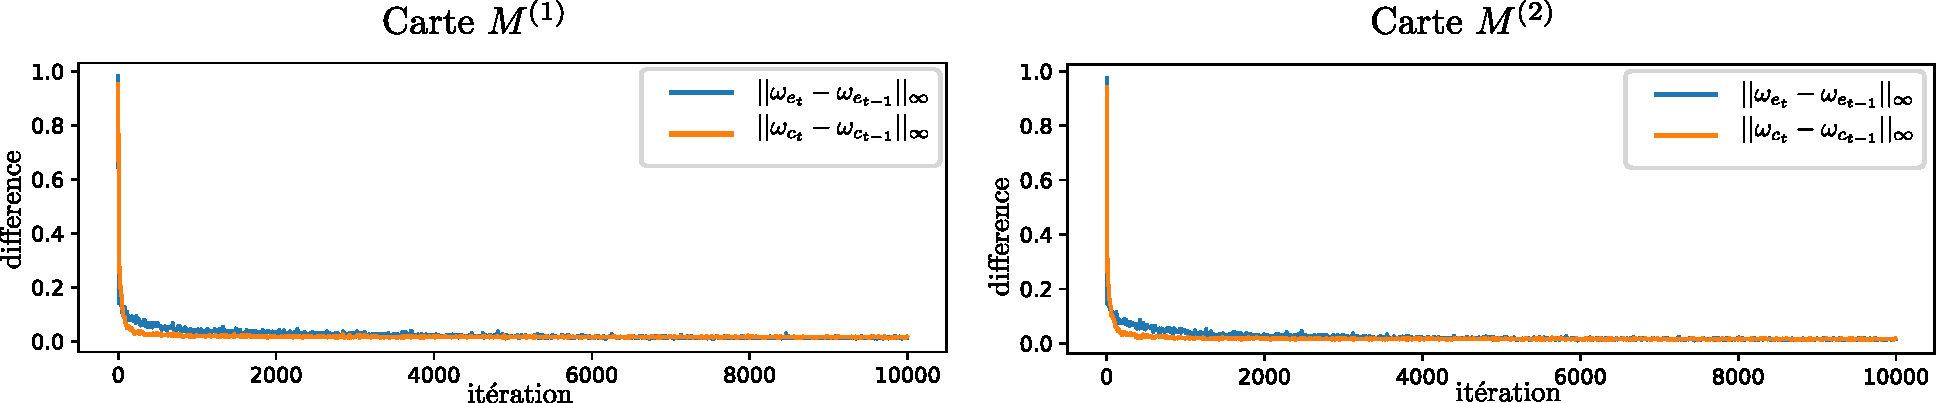
\includegraphics[width=\textwidth]{convergence/cercle_moy.pdf}
	\caption{Pour chaque carte, nous représentons l'évolution en fonction du temps d'apprentissage, de la différence maximale en valeur absolue entre les poids à l'instant $t$ et ceux à $t-100$ $\w_t$ et $\w_{t-100}$. Les entrées sont ici un cercle en deux dimensions. L'évolution est moyennée sur 10 apprentissages dont les entrées sont tirées aléatoirement selon la même distribution, un cercle en deux dimensions.
	Ces tracés montrent que les poids externes et contextuels convergent rapidement vers une position stable.\label{fig:conv}}
\end{figure}


\subsubsection{Disposition des poids}

Analysons à présent à l'organisation des cartes lorsque les poids ont convergé.
Les poids, les entrées et les BMUs associés sont tracés en figure~\ref{fig:w} selon la représentation cartographique décrite au chapitre \ref{chap:repr}.
Les poids externes, en orange, présentent une disposition similaire à ceux observés dans une carte classique : ils sont classés de façon monotone entre 0 et 1.
Les poids contextuels, en bleu, présentent une forme de \og vagues \fg{}. 

En rose et vert, nous traçons la valeur des entrées en fonction des positions de BMUs obtenues lors de la phase de test.
Nous observons que les positions des BMUs dans la carte $M\m{1}$ se répartissent en zones, séparées par des zones mortes dont les n\oe{}uds n'ont jamais été BMUs. C'est une première différence avec une carte classique, pour laquelle toutes les positions seront BMUs lorsque les entrées sont distribuées de façon continue.
Les zones dans lesquelles les n\oe{}uds sont BMUs correspondent aux extrema des poids contextuels et leurs alentours.

\begin{figure}[ht!]
	\centering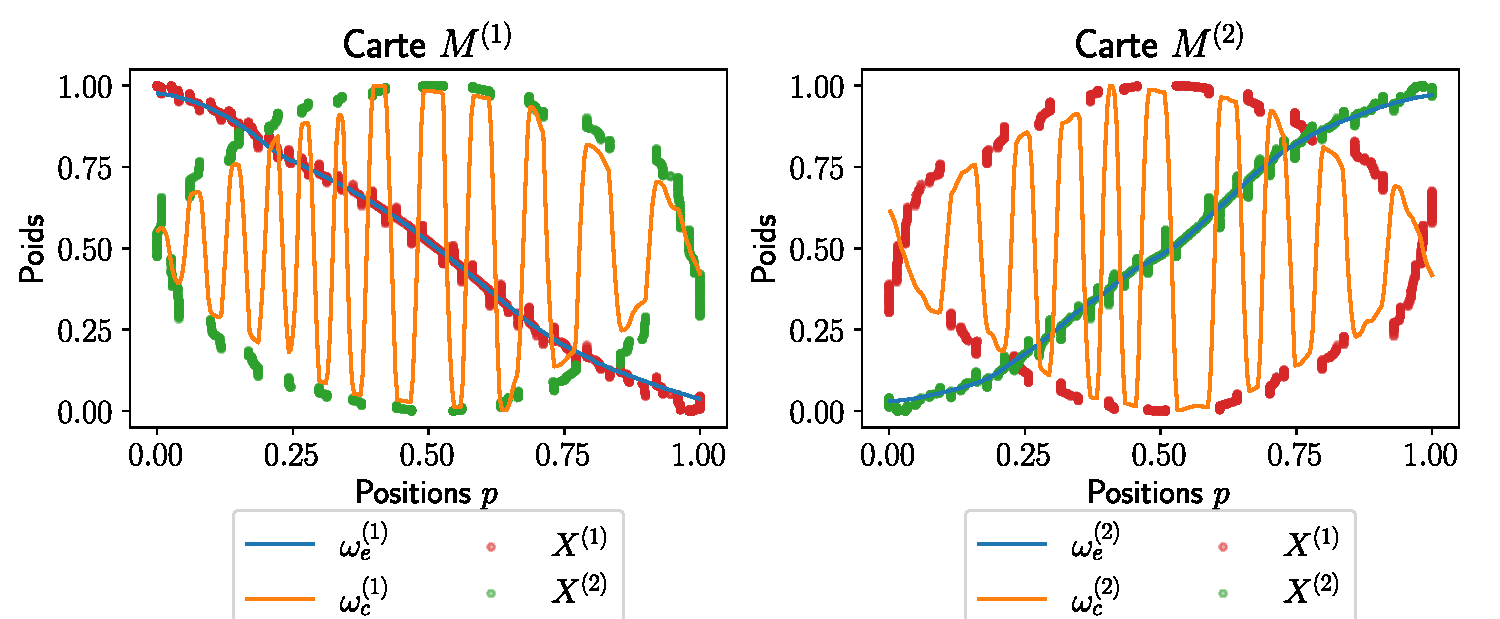
\includegraphics[width=\textwidth]{cercle/weights_500.pdf}
	\caption{Représentation cartographique des poids et entrées lors d'une phase de test selon la position dans chacune des cartes. Nous remarquons que les poids d'une carte, par exemple la carte $M^{(1)}$ s'organisent en zones différenciant les valeurs de la paire $X^{(1)}, X^{(2)}$ et non seulement de la valeur de $X^{(1)}$. Deux zones adjacentes codent pour des valeurs de $X^{(1)}$ proches, mais $X^{(2)}$ différents. Au sein d'une même zone, les BMUs s'organisent sous la forme d'une sous-carte auto-organisée sur les valeurs de l'entrée contextuelle. Ces zones se forment de manière auto-organisée. \label{fig:w}}
\end{figure}

La figure~\ref{fig:w_zoom} est un agrandissement du tracé sur quatre zones de la carte $M\m{1}$.
Elle met en évidence le fait que les zones définies par les poids contextuels se partagent les positions des BMUs en fonction de la valeur des entrées~:
Les deux points représentés en rouge et bleu ont la même valeur de $\inpx\m{1}$ mais une valeur différente de $\inpx\m{2}$. 
Ils ont ici un BMU différent dans la carte $M\m{1}$, et ces BMUs sont situés dans deux zones adjacentes.
Globalement, deux zones adjacentes correspondent à des segments de valeur d'entrée externes qui se recouvrent.

\begin{figure}[h!]
	\centering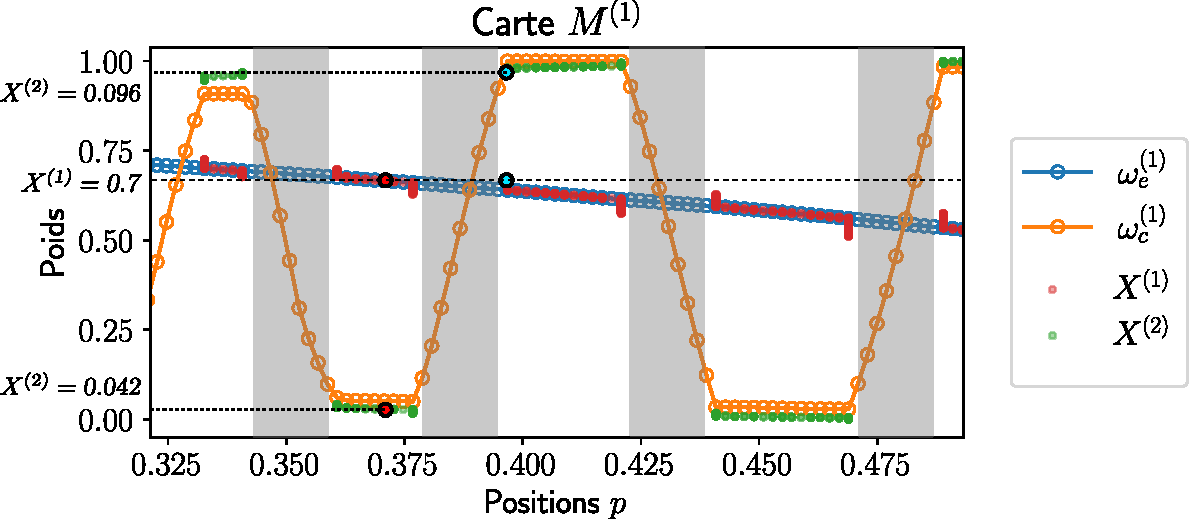
\includegraphics[width=0.7\textwidth]{cercle/weights_zoom_500.pdf}
   \caption{Zoom sur la figure \ref{fig:w} entre les positions 0.35 et 0.55 de la carte $M\m{1}$. 
   Nous y faisons apparaître la position sur la courbe des n\oe{}uds de la carte.
   Deux zones consécutives seront BMUs pour des ensembles d'entrées qui se recouvrent. Par exemple, les deux entrées correspondant au points bleu et rouges ont les mêmes valeurs de $\inpx\m{1}$, mais des valeurs différentes de $\inpx\m{2}$. Leurs BMUs sont alors séparés dans la carte $M\m{1}$ dans deux zones consécutives.
   Entre les zones, quelques unités ne sont jamais BMU, en gris sur la figure. Il s'agit de zones mortes, créant des discontinuités dans la réponse de la carte.
   \label{fig:w_zoom}}
\end{figure}

Dans chaque carte, une position se spécialise donc en tant que BMU par rapport à son entrée externe et à son entrée contextuelle.
Cette différenciation est réalisée par une organisation de la carte en un nombre fini de zones distinctes. Dans chaque zone, les unités sont BMUs pour un segment de valeurs d'entrée externe et contextuelles. Au sein d'une zone, la répartition des entrées externe selon le BMUs est ordonnée, comme ce serait le cas dans une carte auto-organisatrice classique. Le comportement de la carte au sein d'une zone reste donc similaire à celui d'une carte classique.
Il s'agit d'une deuxième échelle d'organisation, qui garde également l'aspect ordonné d'une carte classique. 
Ces zones sont créées par auto-organisation~; aucun paramètre de la carte n'a été modifié pendant l'apprentissage pour former ces zones.

\subsubsection{Erreur de quantification vectorielle}

Nous nous intéressons enfin à la quantification vectorielle réalisée sur l'entrée externe dans chaque carte. 
Nous souhaitons que le poids externe du BMU soit une approximation de l'entrée externe. Cette quantification permet d'interpréter la sortie d'une carte dans l'espace des entrées, par exemple pour prédire une valeur.

La Figure~\ref{fig:qv} présente la valeur de cette approximation au sein de chaque carte, $\w\ext(\bmu\m{i})$, en fonction de l'entrée correspondante $\inpx\m{i}$. 
Cette figure montre que la quantification vectorielle est bien réalisée~: les valeurs approximées sont proches des valeurs d'entrées.
L'erreur de quantification est plus forte que celle qu'on obtiendrait avec une carte de même taille et mêmes paramètres apprenant sur l'ensemble de $\inpx\m{i}$~. 
Nous remarquons enfin une disposition en étages, dues aux zones formées par les poids contextuels.
Les n\oe{}uds de zones adjacentes de la carte sont en effet BMU pour des intervalles d'entrée qui se recoupent.
Une même valeur d'entrée peut avoir un BMU dans deux zones consécutives de la carte en fonction de la valeur de l'entrée contextuelle. Comme les poids externes sont strictement croissants (ou décroissants), cela induit l'erreur observée dans la prédiction d'entrée.

\begin{figure}[h!]
	\centering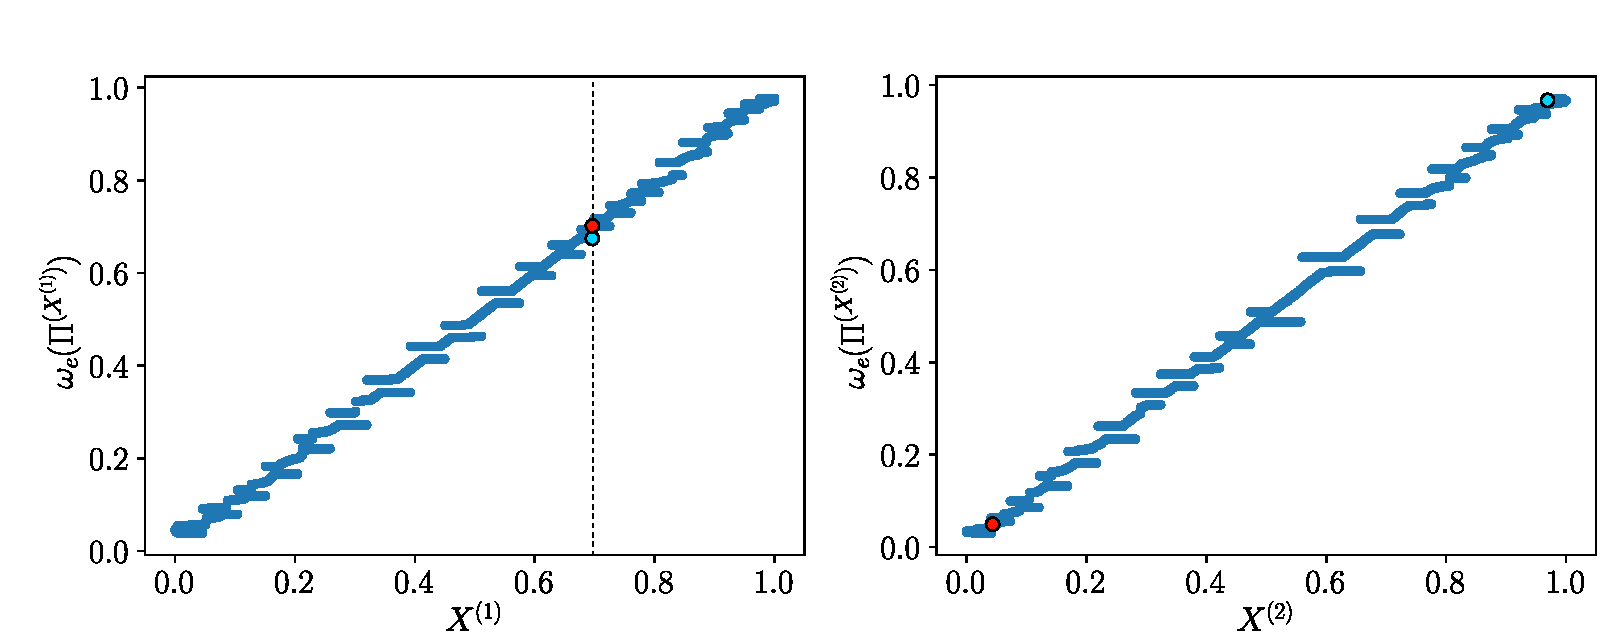
\includegraphics[width=\textwidth]{cercle/frz-error-500.pdf}
	\caption{Représentation de l'erreur de quantification sur les valeurs de $X^{(1)}$ et $X^{(2)}$. Le poids externe du BMU est proche de la valeur de l'entrée~; chaque carte réalise ainsi une bonne quantification vectorielle sur ses entrées. 
	Les poids rouges et bleus représentés en figure \ref{fig:w_zoom} sont reportés sur le graphique. \label{fig:qv}}
\end{figure}

\subsubsection{Apprentissage du modèle dans chaque carte}

Enfin, au \ref{chap:repr}, nous avons observé que l'apprentissage des relations entre entrées se traduit par une relation fonctionnelle entre $U$ et $\bmu$ dans chaque carte, voir figure~\ref{fig:U_BMU}.
Cette propriété traduit l'observation qu'un BMU se spécialise en fonction de l'entrée externe et des entrées contextuelles.

\subsubsection{Résumé des observations}

Les résultats de cette expérience ainsi que les observations présentées au chapitre~\ref{chap:repr} nous permettent donc de formuler les hypothèses suivantes concernant le comportement d'architecture de deux cartes en une dimension~:

\begin{itemize}
	\item Chaque carte de l'architecture présente une faible erreur de quantification vectorielle sur ses entrées externes \ref{fig:qv}
	\item Les poids contextuels de chaque carte s'organisent en zones distinctes. Une zone correspond à un même intervalle de valeur pour $\inpx$ et $U$. Deux zones adjacentes encodent le même intervalle de valeurs de $\inpx$ mais des valeurs distinctes de $U$. Ces zones se caractérisent par un étirement de la carte entre deux valeurs éloignées, apportant un aspect discontinu. Cette discontinuité passe en fait par la présence d'une zone peu dense de la carte contenant des n\oe{}uds qui ne seront jamais BMUs. Nous verrons en section \ref{sec:pred} que la formation de ces zones ainsi que la propriété de quantification vectorielle de l'entrée externe permet à la carte de prédire des entrées manquantes.
	\item L'apprentissage du modèle d'entrée par l'architecture se traduit par l'existence d'une relation fonctionnelle entre $U$ et $\bmu$ dans chaque carte, montrant que chaque carte encode l'état de toute l'architecture et non seulement l'état des entrées externes.
\end{itemize}

Nous chercherons à vérifier ces hypothèses sur d'autres dispositions d'entrées dans des structures de deux cartes et de compléter ces observations.
Nous étudierons si les zones dépendent du modèle d'entrées, comment ces zones se forment et quelles propriétés d'apprentissage elles confèrent à l'architecture de cartes.
Nous introduirons ensuite un comportement possible grâce à l'architecture de cartes~: la prédiction d'entrée manquante.

\subsection{\'Evaluation des hypothèses sur les autres distributions d'entrées}

Nous comparons l'organisation des poids et des BMUs sur les différentes dispositions d'entrées.
Dans toutes ces dispositions, nous avons vérifié que la quantification vectorielle est bien réalisée dans chaque carte sur ses entrées. Nous nous concentrerons sur la présence ou non de zones de poids contextuels dans l'organisation finale des poids en fonction de la distribution des entrées.

La figure \ref{fig:id_results} présente la disposition des poids et entrées des cartes lorsque $\inpx\m{1}$ et $\inpx\m{2}$ sont identiques (Entrées \textbf{C}).
Dans ce cas, les poids externes et contextuels ne forment pas de zones et les deux cartes se comportent comme une seule carte simple sur $\inpx\m{1} = \inpx\m{2}$. 
En figure~\ref{fig:cos_results}, la dépendance entre les entrées présentée n'est bijective~: $\inpx\m{2}$ est fonction de $\inpx\m{1}$, mais pas l'inverse (Entrées \textbf{B}). 
La carte $M\m{1}$ ne forme pas de zones, car une seule valeur de $\inpx\m{2}$ correspond à une même valeur de $\inpx\m{1}$.
Au contraire, la carte $M\m{2}$ doit à présent se diviser pour apprendre les deux valeurs de $\bmu\m{1}$ possibles correspondant à $\inpx\m{2}$. 
Ce comportement rejoint ainsi celui observé sur le cercle.

Regardons maintenant l'organisation des cartes lorsqu'une valeur de $\inpx\m{1}$ correspond à plus de valeurs de $\inpx\m{2}$~: 4 dans le cas de la courbe de Lissajous (Entrées \textbf{B}) ou tout l'intervalle $[0,1]$ dans le cas du patch $[0,1]^2$ (Entrées \textbf{E}). Ces organisations sont tracées en figure~\ref{fig:lissa} et \ref{fig:ind}.
Dans ces deux derniers cas, les cartes présentent encore une organisation en zones des poids contextuels, tout comme le comportement observé sur le cercle. 
Le nombre de zones est similaire à ce qui est observé sur le cercle, alors que la répartition des entrées est différente. Par contre, la forme des zones varie légèrement.
Contrairement au cas précédents, les BMUs se répartissent sur toutes les valeurs de $\w_c$ dans une zone.


Nous pouvons en conclure que la présence de zones est un comportement systématique de la carte étant donné qu'elles sont observées même lorsque les entrées sont indépendantes. 
Cependant, elles émergent de l'organisation seulement lorsque qu'elles sont nécessaires, lorsqu'une carte doit pouvoir différencier au moins deux valeurs d'entrée contextuelles différentes correspondant à une même valeur d'entrée externe.
La forme des zones et la réponse des cartes dépend ensuite de la relation entre entrées.
Sur la distribution indépendante, la carte ne présente pas de zone morte. La totalité d'une zone se déploie de manière à couvrir l'ensemble des valeurs de $U$ correspondant à cette zone, ce qui est également observé en figure ~\ref{fig:lissa} pour les courbes de Lissajous. Une zone agit alors comme une petite carte d'une sous-région de l'espace d'entrée. 

\begin{figure}[H]
	\centering\includegraphics[width=0.8\textwidth]{id/weights.pdf}
	\vspace{-0.3cm}
	\caption{Représentation cartographique des poids et entrées pour la disposition identité. Les poids externes et contextuels sont superposés, et les poids contextuels n'ont pas besoin de former de zones \label{fig:id_results}}
\end{figure}
\begin{figure}[H]
	\centering\includegraphics[width=0.8\textwidth]{cos/weights.pdf}
	\vspace{-0.3cm}
	\caption{Représentation cartographique des poids et entrées pour $\inpx\m{2} = cos(\inpx\m{1}$. Les poids contextuels de la carte $M\m{1}$ ne forment pas de zones car une seule valeur de $\inpx\m{2}$ correspond à une entrée $\inpx\m{1}$. Au contraire, les poids de la carte $M\m{2}$ s'organisent pour gérer la distinction. \label{fig:cos_results}}
\end{figure}
\begin{figure}[H]
	\centering\includegraphics[width=0.8\textwidth]{lissa/weights.pdf}
	\vspace{-0.3cm}
	\caption{Représentation cartographique des poids et entrées pour des entrées sur une courbe de Lissajous. Les poids contextuels se disposent en zones afin de différencier les BMUs selon l'entrée externe et l'entrée contextuelle. Une zone est une carte d'une sous-region des entrées externes \label{fig:lissa}}
\end{figure}

\begin{figure}[ht]
	\centering\includegraphics[width=0.8\textwidth]{square/weights.pdf}
	%\vspace{-0.5cm}
	\caption{Représentation cartographique des poids et entrées dans le patch $[0,1]^2$. Les poids contextuels s'organisent en zones qui cartographient des sous région de l'espace d'entrée. \label{fig:ind}}
\end{figure}

En figure~\ref{fig:2som_p_d}, nous traçons la distorsion des poids externes $(\omega_e(\bmu\m{1}), \omega_e(\bmu\m{2}))$ des cartes correspondant au patch $[0,1]^2$. Ce tracé nous permet de visualiser la quantification vectorielle dans l'espace d'entrée multimodal et non seulement sur chaque carte. 
Nous y observons que les cartes quantifient tout l'espace $[0,1]^2$, mais que seulement une centaine de points servent à la quantification, alors que les deux cartes sont de taille 500. Ces points sont définis par les zones de poids contextuels des cartes. La carte $M\m{1}$ classe ensuite les entrées selon les valeurs de $\inpx\m{1}$ tandis que $M\m{2}$ les classe selon les valeurs de $\inpx\m{2}$. 
\begin{figure}[t]
	\begin{minipage}{0.48\textwidth}
		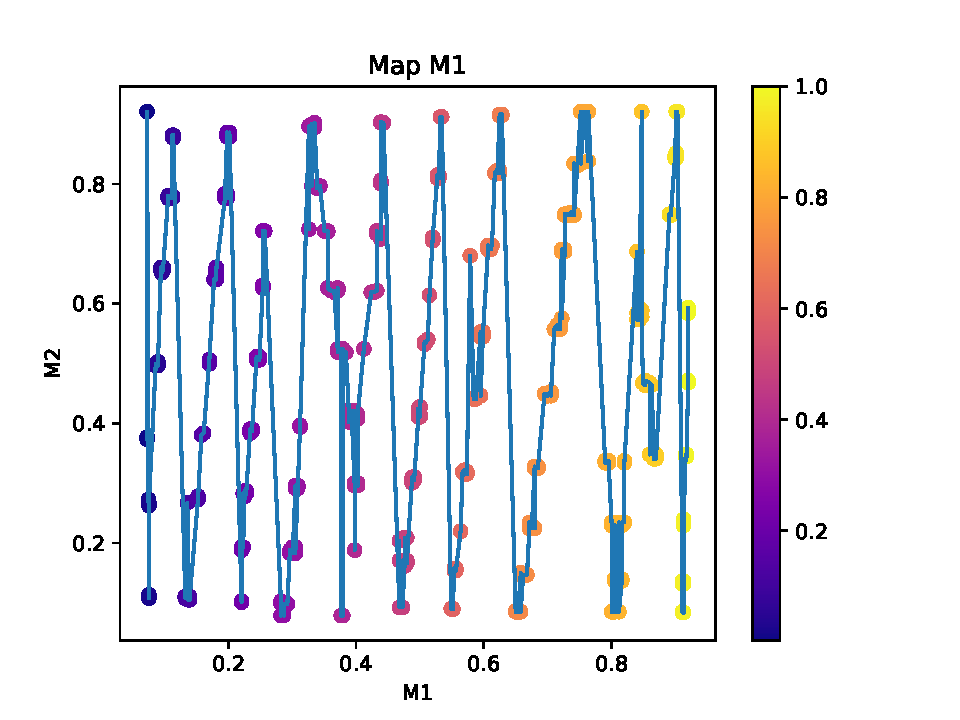
\includegraphics[width=\textwidth]{2som_square_d}
	\end{minipage}
	\begin{minipage}{0.48\textwidth}
		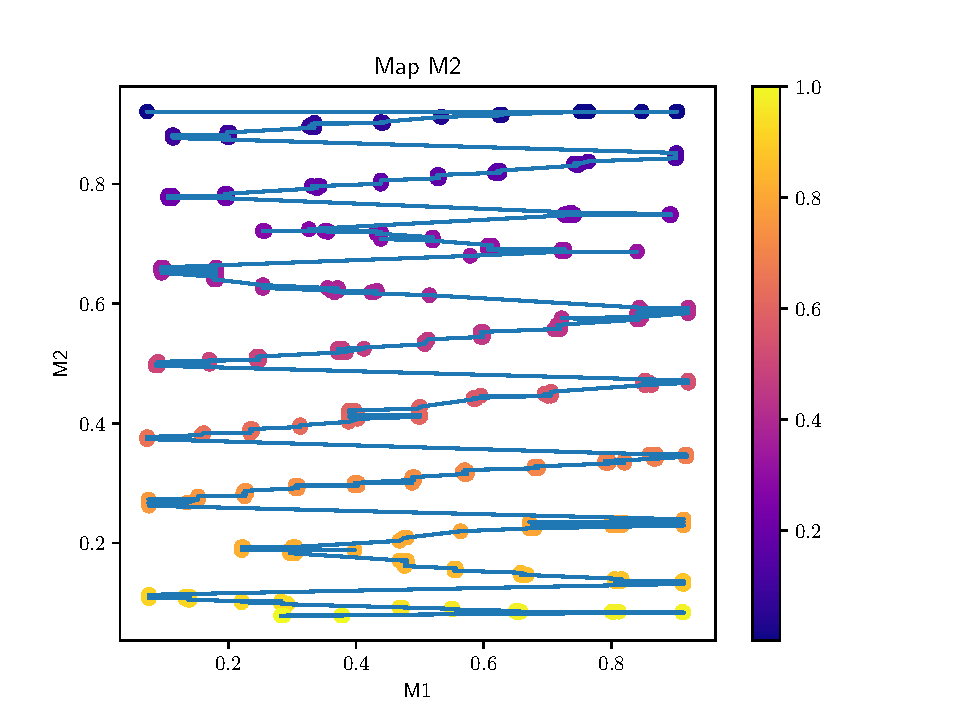
\includegraphics[width=\textwidth]{2som_square_d2}
	\end{minipage}
	\caption{Représentation de la distortion des poids des deux cartes dans l'espace d'entrée $\inpx\m{1}, \inpx\m{2}$ lorsque les entrées sont indépendantes. Les cartes s'organisent de façon à quadriller le carré, l'une selon les $\inpx\m{1}$, l'autre selon les $\inpx\m{2}$. Bien que chaque carte a 500 n\oe{}uds, on observe seulement environ 90 valeurs possibles pour les paires $\w_e(\bmu\m{1}),\w_e(\bmu\m{2})$ \label{fig:2som_p_d}}
\end{figure}

Enfin, nous voulons vérifier si les cartes sont robustes au bruit en prenant des données en forme d'anneau (Entrées~\textbf{(E)}), représentées en Figure~\ref{fig:anneau_w}. La disposition des poids et entrées rejoint les observations réalisées sur les autres expériences.
Nous ajoutons que, dans toutes ces dispositions d'entrées le tracé de $U$ en fonction de la position du BMU dans chaque carte montre une relation fonctionnelle entre $U$ et les positions du BMU, ce qui montre que chaque carte de l'architecture a appris une représentation du modèle d'entrée. Nous reviendrons plus en détail sur l'utilisation de $U$ dans l'analyse des réponses des cartes au chapitre \ref{chap:indicateur}.
\begin{figure}[H]
	\centering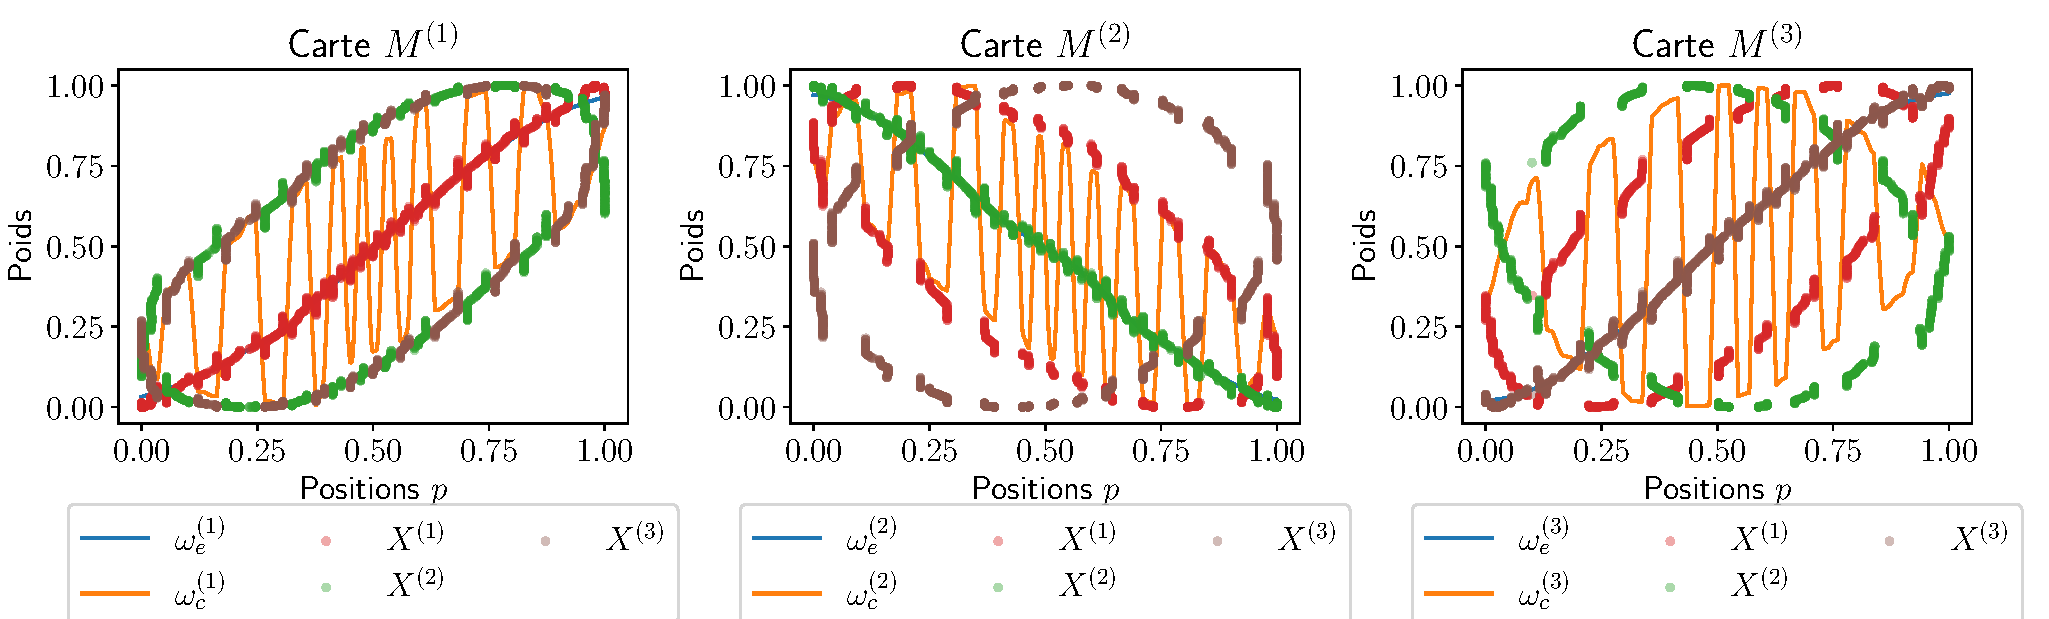
\includegraphics[width=0.8\textwidth]{anneau/weights_001.pdf}
	\caption{Représentation cartographique des poids et entrées pour des entrées sur un anneau. \label{fig:anneau_w}}
\end{figure}

\subsection{Mécanismes de formation des zones de poids contextuels}

L'organisation en zones observée sur les distributions d'entrées en 2D confirment et complètent les hypothèses formulées sur la disposition d'entrées en cercle~:
Les poids des cartes s'organisent en fonction de l'entrée externe, puis des zones se forment systématiquement pour différencier le modèle latent. Les zones se forment dès lors que plusieurs valeurs d'entrées contextuelles correspondent à une même valeur d'entrée externe dans une carte.
L'organisation et le nombre de zones sont ensuite liées aux mécanismes d'apprentissage de la carte.
Nous nous intéressons à quelques mécanismes des cartes influençant la formation de zones. 
Nous comparerons ainsi l'organisation obtenue sur une même disposition d'entrées, pour différents couples de rayons de voisinage contextuels et externes. 
Nous regarderons ensuite si les zones ont une influence sur la convergence de la relaxation.

\subsubsection{Dépendance aux paramètres des cartes}

Nous voulons observer comment les zones dépendent des paramètres de l'architecture, en particulier des rayons externes et contextuels.
Nous reprenons les entrées \textbf{A}, en cercle et lançons l'apprentissage de plusieurs architectures, de paramètres différents. $r_e$ est fixé à $0.2$ et $r_c$ varie de $0.2$ à $0.005$. 

En figure \ref{fig:rcre}, nous traçons la représentation cartographique de $M\m{1}$ après apprentissage pour ces différents rayons de voisinages. 
Nous n'avons pas représenté $M\m{2}$, mais son comportement est semblable à $M\m{1}$ par la symétrie des entrées.
Notons également que nous avons observé que l'organisation dépend bien du rapport entre rayons de voisinage et non de la valeur du rayon de voisinage contextuel en elle-même. C'est pourquoi nous fixons $r_e$ à $0.2$ sur cet exemple et faisons seulement varier $r_c$.

Pour $r_c = r_e$, ainsi que $r_c \geq r_e$, la carte ne s'organise pas en zones. 
La formation de celles-ci intervient pour $r_c < r_e$. Sur la figure, nous commençons à voir des zones de poids contextuels apparaître pour $r_e = 3r_c$, sans que les BMUs ne marquent de séparation. La notion de zones est observée pour $r_e = 4r_c$.
Le nombre de zones de BMU augmente ensuite avec le rapport des rayons de voisinage. La taille du rayon de voisinage contextuel est ensuite limité par la taille de la carte. Si celui-ci est trop faible, la notion de zone de poids contextuel n'a plus lieu d'être. C'est ce qu'on observe pour $\frac{r_e}{r_c} = 40$. $r_c$ est de $2$ unités. Chaque zone de BMU ne compte que quelques unités, on ne peut donc plus vraiment parler de sous-carte.

\begin{figure}[H]
	\includegraphics[width=\textwidth]{rceqre/rcre_tot.pdf}
	\caption{Représentation cartographique de la carte $M\m{1}$ pour différents rayons de voisinage contextuels, le rayon de voisinage $r_e$ étant fixé à $0.2$. Nous observons que la présence de zones dépend du rapport entre les rayons de voisinage. La carte définit des zones de BMUs grâce à la forme poids contextuels, de plus en plus nombreuses et contenant de moins en moins d'unités lorsqu'on augmente le rapport entre rayons de voisinage.
	La carte $M\m{2}$, non représentée ici, se comporte de façon similaire.\label{fig:rcre}
	}
\end{figure}	

En faisant la même expérience pour les autres dispositions d'entrées, nous pouvons observer que pour un même couple $r_e,r_c$, le nombre de zones reste similaire quelle que soit l'expérience. Leur forme diffère en fonction des entrées.
C'est bien les paramètres des cartes qui induisent donc l'organisation en zones.
L'organisation au sein d'une zone et la forme des poids contextuels dépendent ensuite du modèle d'entrées.

Ces zones peuvent s'expliquer du fait que le rapport entre rayons de voisinage introduit une relation subordonnée entre les poids lors de la mise à jour ainsi que deux échelles temporelles de mise à jour. 
Les poids externes se déplient en effet plus vite que les poids contextuels, puis gardent une \og attraction \fg{} plus forte sur les unités voisines. Les poids contextuels doivent donc composer avec cette force.

Les rayons de voisinage sont les paramètres ayant le plus d'influence sur l'organisation des cartes, d'où le choix de les étudier.
Dans nos expériences, nous avons pris $r_c$ identique pour toutes les couches de poids contextuels.
Nous pourrions cependant associer à chaque couche de poids d'une carte un rayon de voisinage différent. 
Enfin, nous pouvons aussi faire varier le taux d'apprentissage $\alpha$, ainsi que les paramètres de la fonction d'activation $\beta$, $\sigma$, etc.
Pour pouvoir adpater ces paramètres automatiquement dans un objectif d'application et réaliser une étude paramétrique approfondie, il nous faudrait définir une fonction de coût caractérisant l'organisation d'une carte ou relative à un objectif d'apprentissage. 
Nous discuterons d'un tel indicateur au chapitre \ref{chap:indicateur}, mais soulignons ici que nous n'avons pas encore défini de valeur adéquate. 
C'est pourquoi nous nous sommes intéressés à la compréhension de l'effet des paramètres dans nos travaux actuels, et n'avons pas cherché à optimiser ces valeurs.


\subsubsection{Influence de la présence de zones sur la recherche de BMU par relaxation}

Nous nous intéressons au passage à l'influence de la formation de zones sur le processus de relaxation.
Nous pourrions penser que ces zones favorisent la recherche de consensus lors de la relaxation et la convergence des poids.
Nous traçons en figure~\ref{fig:conv_rcre} le nombre de pas moyen nécessaire à la recherche du BMU par relaxation et les indicateurs de convergence des poids des cartes, dans le cas d'une carte ayant formé des zones et d'une carte n'en ayant pas formé ($\frac{r_e}{r_c} = 1$). 
Ces valeurs sont similaires dans les deux cas.
Sur des cartes 1D, nous n'observons donc pas d'amélioration de la relaxation grâce à la formation de zones.
Cela montre que la convergence de la relaxation n'est pas spécifique aux valeurs de paramètres choisies dans ces expériences et est ainsi une méthode générale de connexion entre cartes.

\begin{figure}[hb]
	\centering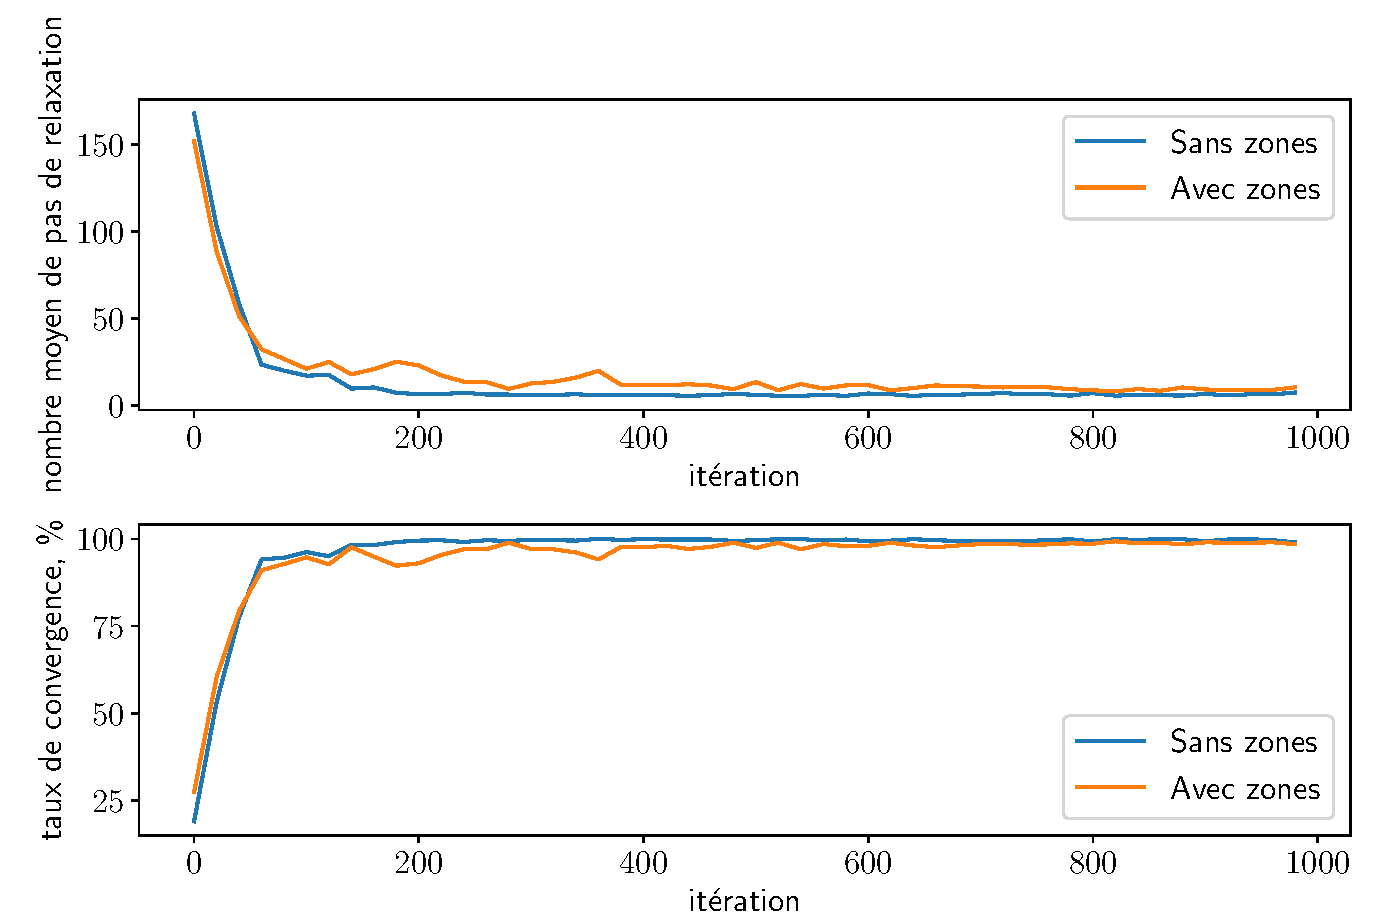
\includegraphics[width=0.8\textwidth]{rceqre/convergence_relax.pdf}
	\caption{\'Evolution du nombre moyen de pas de relaxation et du taux de convergence pour une organisation de cartes ayant formé des zones de poids contextuels ($\frac{r_e}{r_c} = 10$ ) et une organisation n'ayant pas formé de zones ($\frac{r_e}{r_c} = 1$). Dans les deux cas, la relaxation mène à un consensus en fin d'apprentissage.
	Donc, dans des cartes en une dimension, la formation de zones ne favorise pas significativement la convergence de la relaxation. Par ailleurs, le mécanisme de relaxation a donc un sens général, quels que soient les paramètres des cartes. \label{fig:conv_rcre}}
\end{figure}

\subsection{Discussion}

Les motifs en zones formés par les poids contextuels sont un mécanisme qui émerge du processus d'évolution des cartes. Ces zones dépendent principalement des rayons de voisinages.
Au sein d'une même zone, les poids externes ont des valeurs très proches et les poids contextuels s'organisent de manière à former une sous-carte des valeurs possibles de l'entrée contextuelle pour un même intervalle de valeurs d'entrée externe.
On pourrait donc introduire une notion d'indices primaires et secondaires dans la carte, l'indice primaire étant celui de la zone et l'indice secondaire la position dans la zone.


Cette notion d'indices primaires et secondaires est observée en biologie dans le cerveau. 
Ainsi la figure~\ref{fig:ballard} présente un schéma d'organisation des neurones du cortex V1 décrit en \cite{ballard_cortical_1986}.
Les auteurs observent que des neurones situés à différents emplacements sur le cortex visuel ne reçoivent pas la même partie du champ de vision, et leur emplacement correspond à la partie du champ de vision traitée (gauche - droite, etc).
Ces entrées différenciées forment une indexation~\emph{primaire} de V1. 
Au sein d'une zone de même indice primaire, les neurones s'organisent alors de façon à représenter tout le sous-espace des entrées ayant été présenté à la zone. Cette sous-carte définit alors des indices secondaires.
Ici, la même entrée est certes présentée à toute la carte, donc la proximité avec ce modèle biologique est limitée. On peut quand même noter qu'après apprentissage, un n\oe{}ud de la carte ne réagit qu'à un sous-ensemble d'entrées définies par les valeurs des poids externes autour cet emplacement, ce qui se rapproche de ce phénomène de spécialisation.


\begin{figure}[H]
	\centering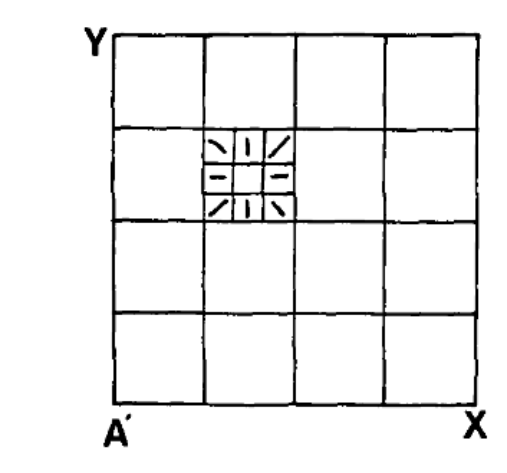
\includegraphics[width=0.3\textwidth]{ballard_primary_secondary.png}
	\caption{Schématisation d'une répartition en indices primaires et secondaire des neurones d'une aire corticale, tirée de~\cite{ballard_cortical_1986}. 
	Les auteurs observent que la réponse de neurones du cortex est organisée en zones selon leur position, formant des indices primaires. Les carrés de la figure représentent cette première indexation.
	Ces zones reçoivent différentes portions de l'espace d'entrée~: les zones situées à gauche du cortex traitent les signaux venant du champ visuel de gauche et ainsi de suite pour couvrir tout le champ visuel.
	Au sein d'une zone, les neurones cartographient toutes les valeurs possibles de l'entrée sous forme de carte topologiquement ordonnée, formant une indexation secondaire. \label{fig:ballard}}
\end{figure}


D'un point de vue computationnel, l'organisation d'une carte se rapproche d'une méthode de modulation~: la valeur de l'activité externe est modulée par l'activité contextuelle. 
La forme des poids permet à cette modulation d'encoder en une seule valeur $X$ et $U$, le modèle d'entrée. Elle émerge de la dynamique d'apprentissage des cartes.

Les zones forment ainsi un deuxième niveau de quantification vectorielle au sein d'une carte. 
Ces deux niveaux de quantifications encodent à la fois l'entrée $\inpx$ et le modèle $U$ en une seule position de BMU.

\section{Génération de modalité dans des architectures de trois cartes 1D}

\subsection{Introduction}

Nous avons vu que dans une architecture de deux cartes, apprenant sur un modèle d'entrée liées tel que le cercle en 2D, chaque carte encode à la fois la valeur de son entrée externe et le paramètre du modèle, $U$, réalisant ainsi un apprentissage associatif. 
Nous voulons maintenant qu'une architecture de cartes soit directement capable d'utiliser cet encodage du modèle d'entrée dans une tâche de génération de modalité manquante après apprentissage.
Même sans qu'une entrée externe ne lui soit présentée, une carte de l'architecture possède une activité contextuelle et donc un BMU. 
Sur l'architecture de deux cartes, il est envisageable de ne pas présenter $\inpx\m{2}$ à la carte $M\m{2}$. La carte $M\m{2}$ aura quand même un BMU défini seulement grâce aux entrées contextuelles, et dont le poids externe $\w_e(\bmu\m{2})$ appartient à l'espace de la modalité $\inpx\m{2}$. 
La valeur $\w_e(\bmu\m{2})$ peut alors être considérée comme une génération de modalité. 


Pour faciliter l'étude de ce comportement, nous nous plaçons dans un cadre de génération d'entrée sur des modèles d'entrée dont la valeur de l'entrée $\inpx\m{p}$ qui n'est pas présentée à l'architecture est complètement déterminée par l'ensemble des autres entrées $\inpx\m{i}$. La valeur générée par l'architecture $\w_e(\bmu\m{p})$ est alors une prédiction de l'entrée manquante.
En comparant la valeur générée, à la valeur théorique de l'entrée, ce cas d'étude nous permettra de vérifier facilement que l'architecture de carte utilise bien le modèle d'entrée qu'elle a encodé pour générer la modalité manquante.
Dans le cas du cercle en 2D, il y a deux valeurs possibles $\inpx\m{2}$ pour une même valeur de $\inpx\m{1}$, donc il manque de l'information pour faire de la prédiction.
Nous nous intéressons plutôt dans cette partie à des modèles d'entrées en trois dimensions dans lesquels la connaissance de $\inpx\m{1}$ et $\inpx\m{2}$ détermine la valeur de la troisième entrée $\inpx\m{3}$.
Nous avons choisi d'étudier des modèles en trois dimensions plutôt que de rester sur des modèles en deux dimensions, afin de vérifier au passage si les propriétés d'organisation observées sur deux cartes s'appliquent également sur une architecture de trois cartes.
Nous construirons ainsi des architectures de trois cartes sur ces modèles d'entrées 3D et étudierons si après apprentissage de toutes les modalités, l'architecture est capable de générer une prédiction précise de la valeur de la modalité manquante à partir des deux modalités présentées.

Cette capacité de génération d'entrée peut constituer un cadre applicatif, par exemple lorsqu'un capteur serait manquant en robotique. Elle nous permettra également de valider l'encodage du modèle par une architecture de cartes.

\subsection{Méthode expérimentale}

Les tâches de prédiction de ce chapitre seront réalisées sur une architecture de trois cartes 1D, toutes connectées entre elles~; cette architecture est représentée en figure~\ref{fig:archi_3maps}.
Chacune des trois cartes prend une entrée externe en une dimension et deux entrées contextuelles qui sont les positions des BMUs des deux autres cartes. Elle possède donc deux couches contextuelles $\w_{c_0}$ et $\w_{c_1}$.

\begin{figure}
	\centering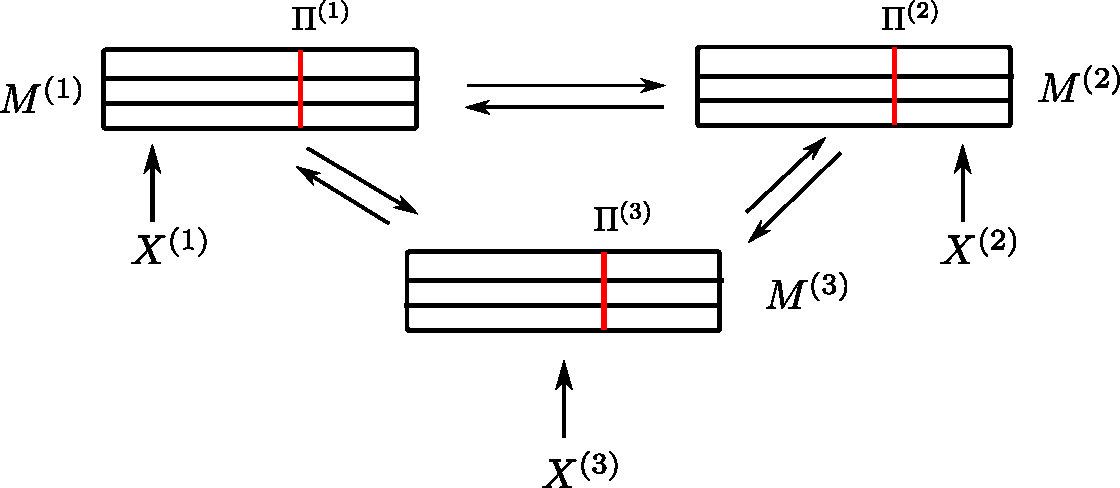
\includegraphics[width=0.8\textwidth]{archi_3maps.pdf}
	\caption{Architecture de trois cartes utilisée dans les expériences. Chaque carte prend une entrée externe $\inpx\m{i}$ et est connectée aux deux autres. Elle possède ainsi deux couches de poids contextuels et une couche de poids externes.\label{fig:archi_3maps}}
\end{figure}

Nous reprenons les modèles d'entrées du cercle 2D et du patch $[0,1]^2$ et choisissons de leur ajouter une troisième dimension, de telle sorte à ce que la connaissance de deux entrées sur trois détermine la valeur de la troisième entrée. Pour cela, nous pivotons le plan 2D de ces entrées dans un espace en trois dimensions.
Ces entrées sont tracées en figure~\ref{fig:inputs_3D}.
Chaque carte de l'architecture prend en entrée une des coordonnées des points 3D du modèle.

L'architecture de deux cartes ayant appris sur le cercle était capable de réaliser une quantification vectorielle précise de l'entrée externe. Nous nous attendons donc à une bonne prédiction sur trois cartes dans le cas du modèle d'entrée \textbf{H}. Dans le cas du plan, la quantification vectorielle sur l'entrée externe était moins précise~: les cartes distinguent une centaine de points sur le plan. 

\begin{figure}[h!]
	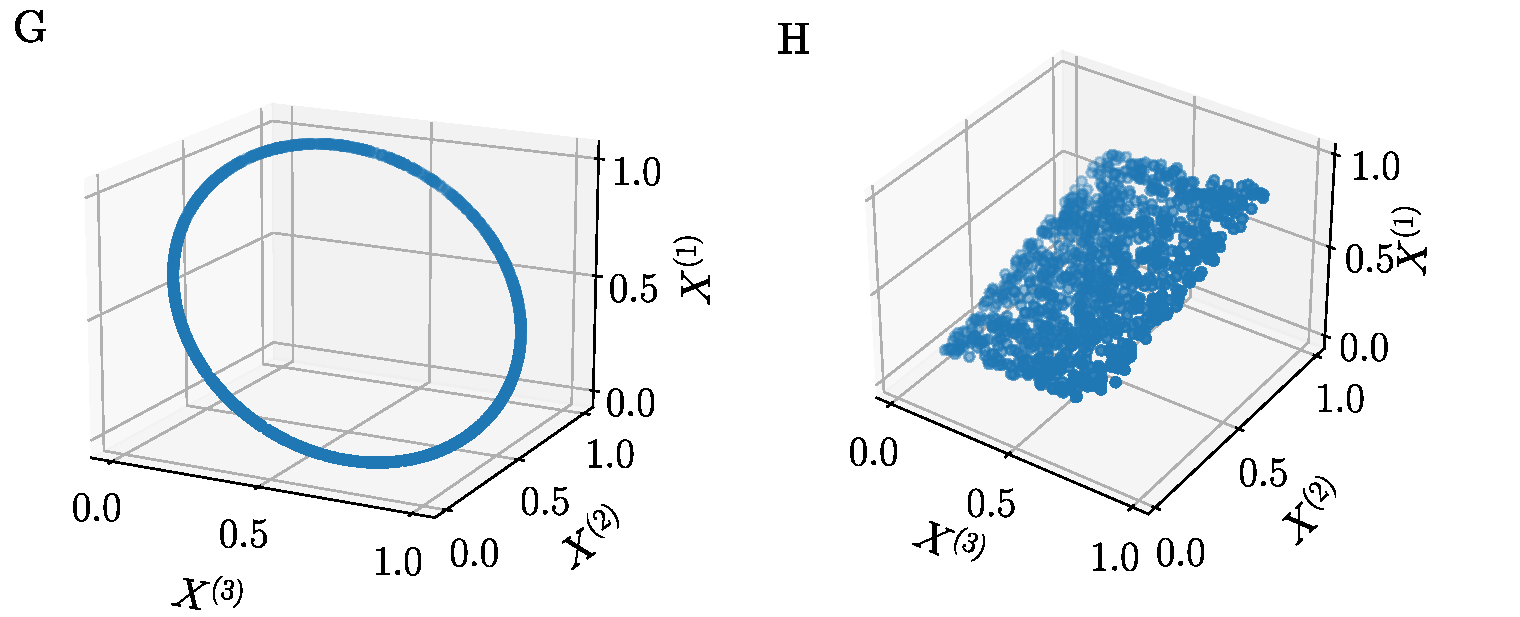
\includegraphics[width=\textwidth]{inputs/inputs_3D.pdf}
	\caption{Dispositions d'entrées en trois dimensions utilisées dans cette partie. Chaque carte $M\m{1}$, $M\m{2}$, $M\m{3}$,prend en entrée une coordonnée $\inpx\m{1}, \inpx\m{2}, \inpx\m{3}$. \label{fig:inputs_3D}}
\end{figure}

L'algorithme de prédiction d'entrée est schématisé en Figure~\ref{fig:schema_pred}.
La phase d'apprentissage du modèle est la même que dans les expériences précédentes~: les trois cartes reçoivent leurs entrées externes $\inpx\m{1},\inpx\m{2}, \inpx\m{3} $
La phase de prédiction est une phase de test, durant laquelle les poids de toutes les cartes ne sont pas mis à jour.
Pour cette phase de prédiction, nous choisissons la carte $M\m{1}$ comme carte prédictive. 
Cette carte ne reçoit plus son entrée externe, mais seulement ses entrées contextuelles. Les autres cartes reçoivent toutes leurs entrées.
La seule différence avec une phase de test classique est que la carte prédictive $M\m{1}$ prend comme activité globale sa seule activité contextuelle. Si la carte possède plusieurs couches de poids contextuels, il s'agit de la moyenne des activités contextuelles.
Nous choisissons comme valeur de prédiction le poids externe du BMU de la carte prédictive $\w\ext\m{1}(\bmu\m{1})$.

Pour les deux modèles d'entrées, nous tracerons la disposition des poids externes et contextuels après apprentissage et vérifierons si les poids contextuels définissent également des zones de BMUs dans chaque carte.
Nous effectuerons dans chaque cas une phase de prédiction de l'entrée $\inpx\m{1}$ et vérifierons si la valeur prédite $\w_e(\bmu\m{1})$ est proche de la valeur attendue $\inpx\m{1}$, qui n'a pas été présentée à la carte.

\begin{figure}
	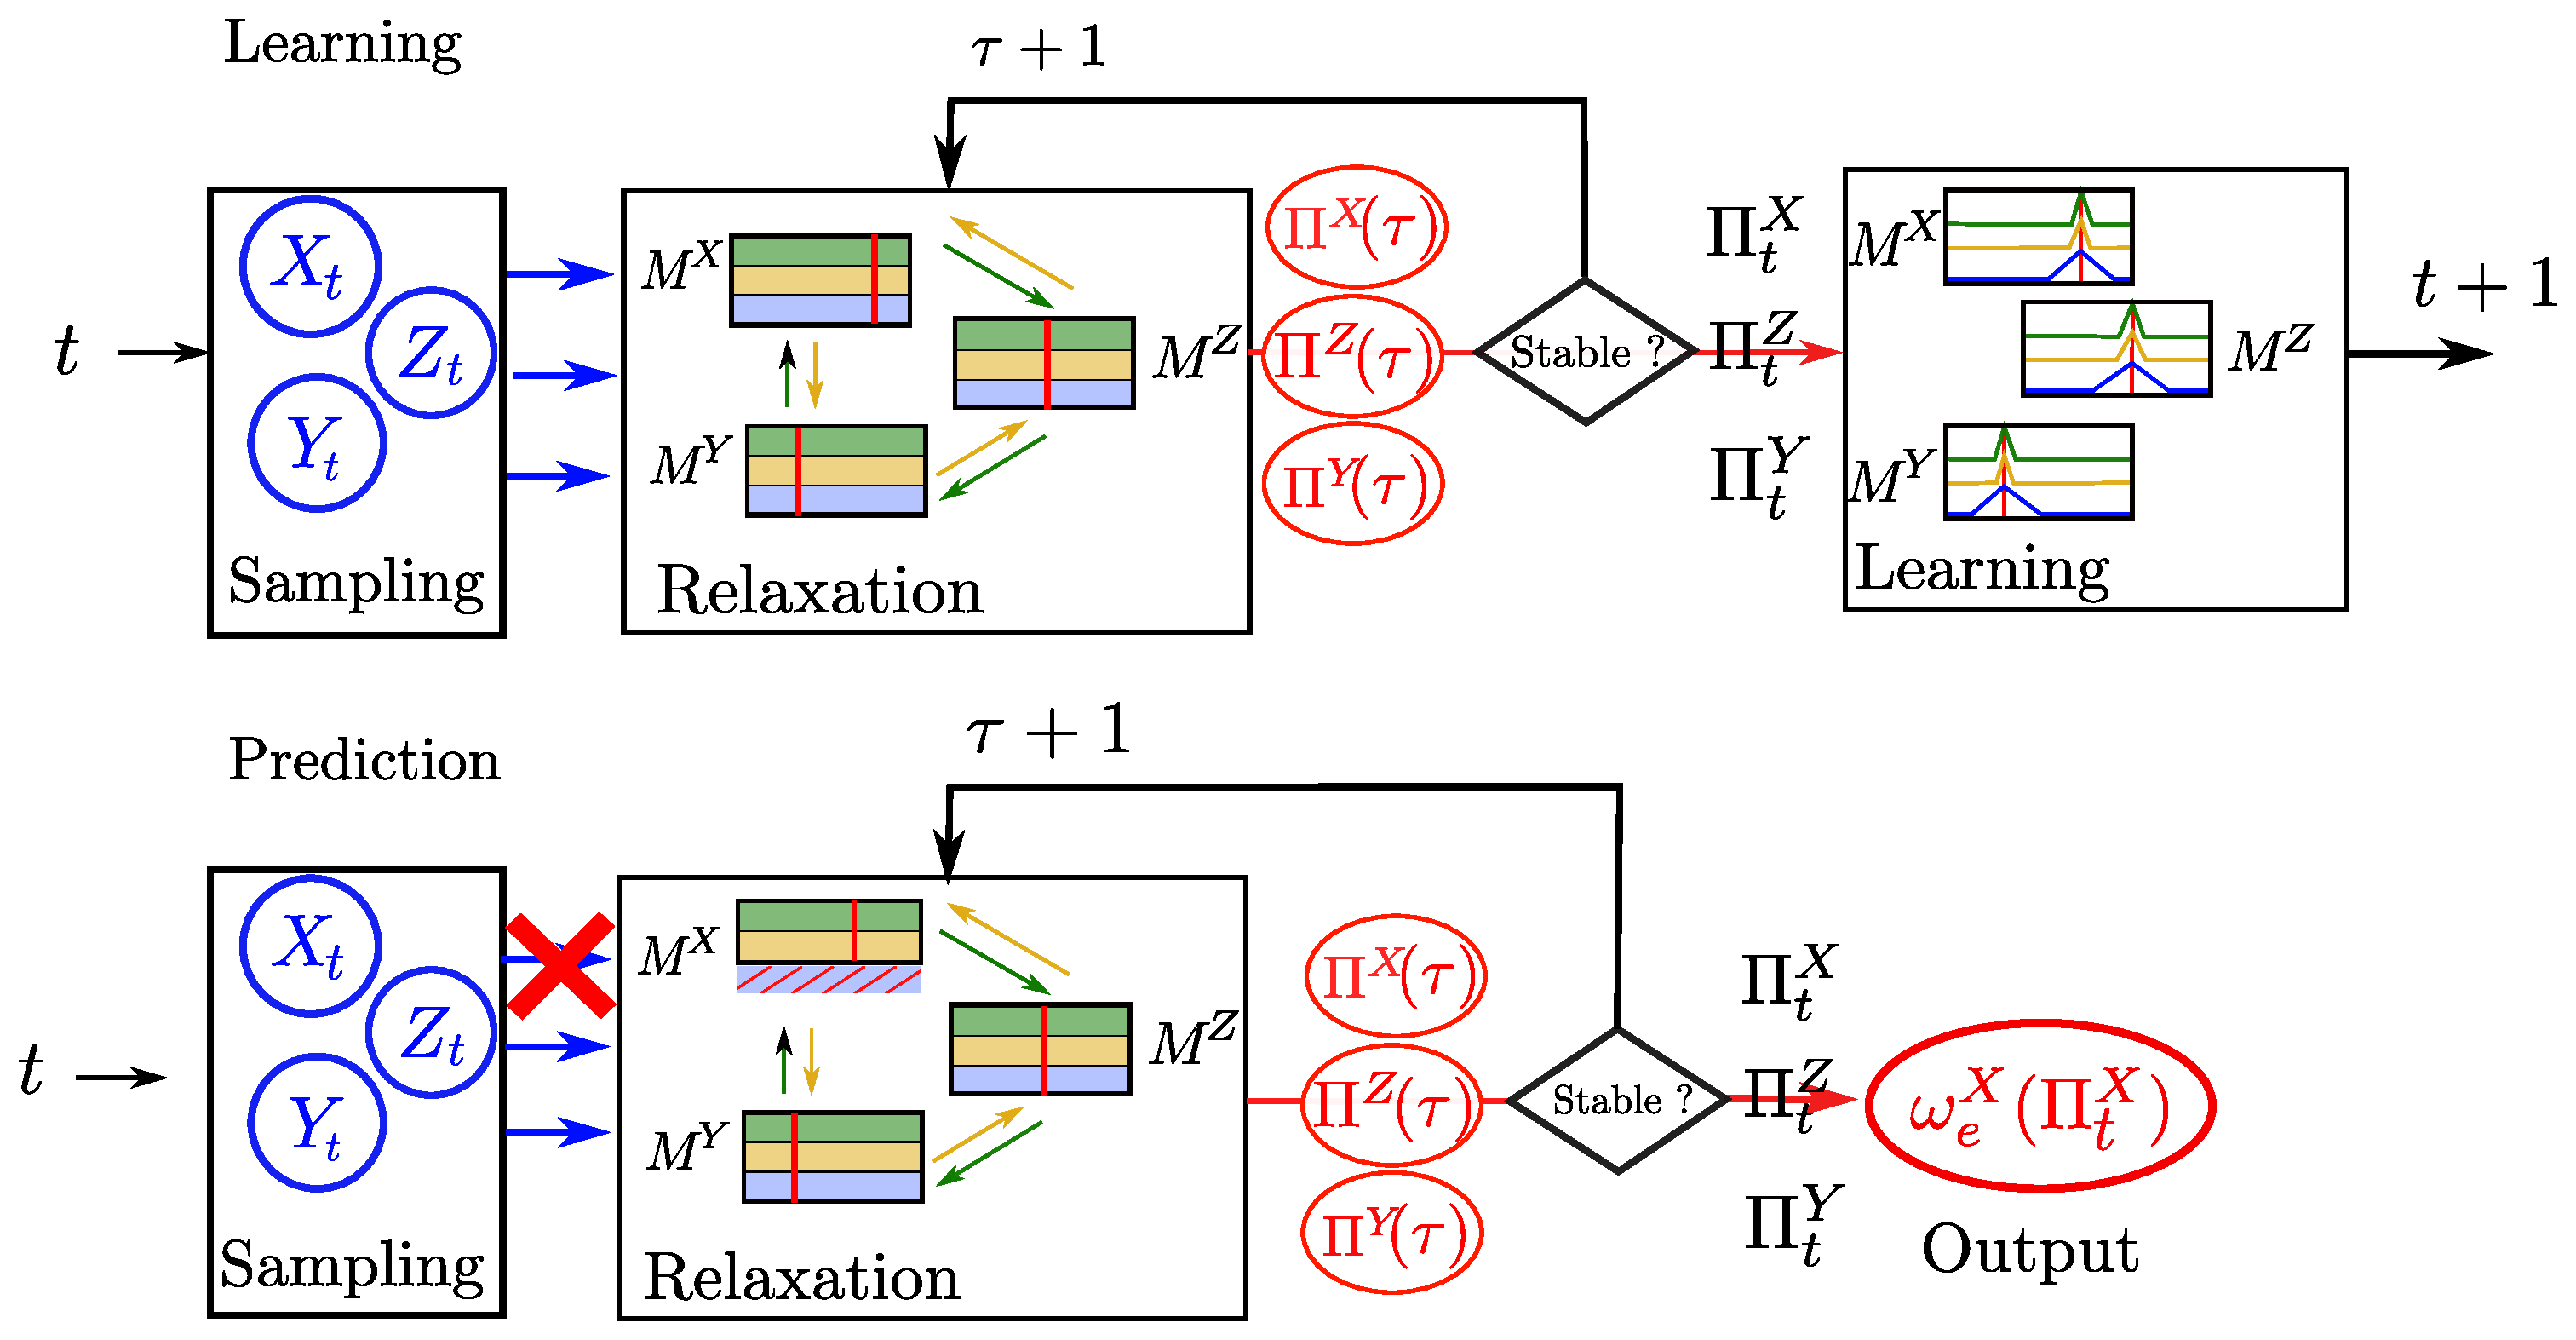
\includegraphics[width=\textwidth]{learning_tests.pdf}
	\caption{Schéma descriptif des opérations effectuées lors de l'apprentissage et de la phase de prédiction.\label{fig:schema_pred}}
\end{figure}

\subsection{Résultats}

Nous traçons en figures \ref{fig:w_cercle} et \ref{fig:w_plan3} la disposition des poids des trois cartes de l'architecture après apprentissage ainsi que des entrées associées pour les entrées dans le cercle 3D (\textbf{G}) et dans le plan 3D (\textbf{H}).
Comme dans la version à deux cartes, les poids contextuels s'organisent en plusieurs zones au sein desquelles la valeur de $U$ est située dans une même plage de valeur. Les deux couches de poids contextuels forment les mêmes zones.
Nous concluons de ces deux tracés qu'une architecture de trois cartes se comporte de la même façon qu'une architecture de deux cartes.

\begin{figure}[h!]
	\centering\includegraphics[width=\textwidth]{cercle3D/weights.pdf}
	\caption{Représentation cartographique des poids et entrées dans l'architecture de trois cartes apprenant sur un cercle en trois dimensions. Nous observons la formation de zones similaires au cas en deux dimensions. \label{fig:w_cercle}}
\end{figure}

\begin{figure}[h!]
	\centering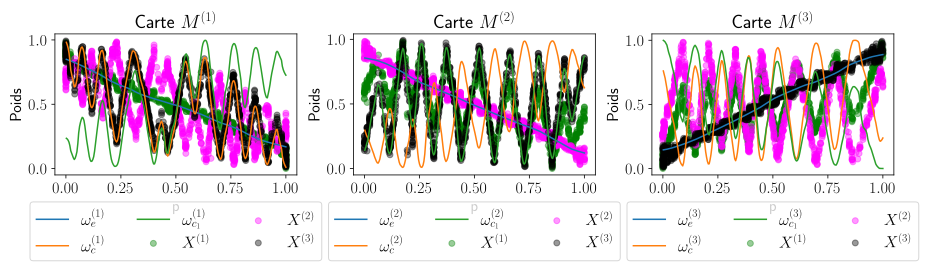
\includegraphics[width=\textwidth]{plan/weights_P2}
	\caption{Représentation cartographique des poids et entrées dans l'architecture de trois cartes apprenant sur un plan pivoté en 3D. Les zones sont similaires au cas en deux dimensions. \label{fig:w_plan3}}
\end{figure}

Nous traçons ensuite l'erreur obtenue lors de la phase de prédiction de $\inpx\m{1}$~: en figure \ref{fig:pred_cercle} pour le modèle du cercle \textbf{G}, et \ref{fig:pred_plan} sur le plan \textbf{H}.
Dans les deux cas, l'entrée $\inpx\m{1}$ n'a pas été présentée à la carte et sa valeur est prédite par $\w\ext\m{1}{\bmu\m{1}}$. Nous ajoutons aux tracés l'erreur de quantification vectorielle dans les autres cartes afin de comparer la qualité de la prédiction à la qualité de la quantification vectorielle.
Nous observons que la prédiction est très bien réalisée dans le cas du cercle. Les valeurs prédites par la carte $M\m{1}$ sont aussi précises que les valeurs quantifiées par les cartes $M\m{2}$ et $M\m{3}$.
L'architecture de cartes a donc encodé le modèle d'entrée et est capable de prédire l'entrée manquante.

Dans le cas du plan, la prédiction est également bien réalisée. L'encodage de $U$ était alors plus large que dans le cas du cercle. Cet encodage plus large se manifeste sur l'intervalle d'erreur prédiction.

\begin{figure}
	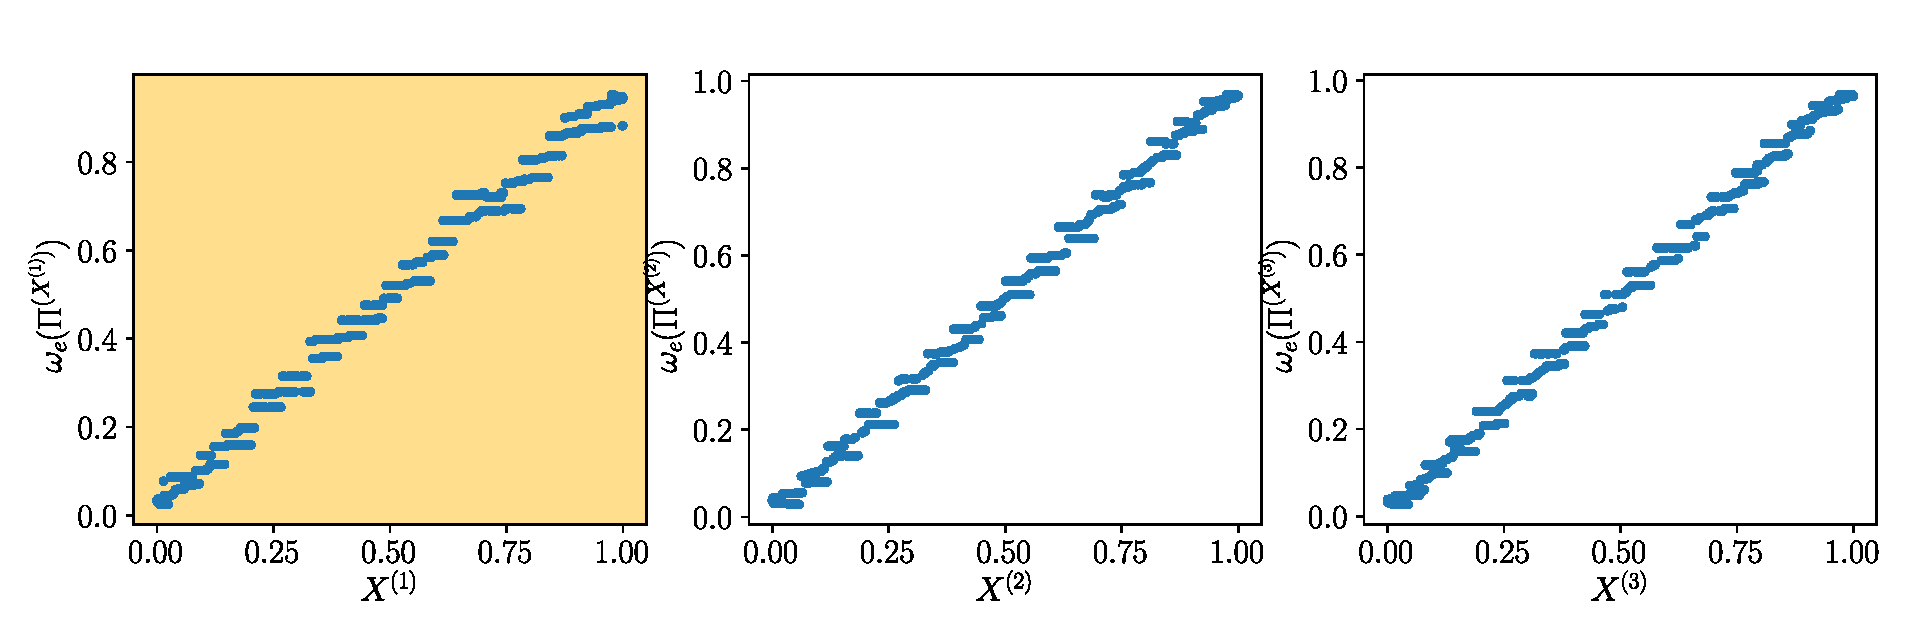
\includegraphics[width=0.95\textwidth]{cercle3D/error-closed-2.pdf}
	\caption{Erreur de prédiction de $\inpx\m{1}$ par $\w_e(\bmu\m{1})$ lorsque les entrées sont sur un cercle en trois dimensions. $\inpx\m{1}$ n'a pas été présenté à $M\m{1}$.
	 Les nuages de points correspondant à $M\m{2}$ et $M\m{3}$ correspondent à l'erreur de quantification dans les cartes 2 et 3 qui ont reçu leur entrée externe. Ces tracés montrent une bonne prédiction de $\inpx\m{1}$ par la carte 1. \label{fig:pred_cercle}}
\end{figure}

\begin{figure}
	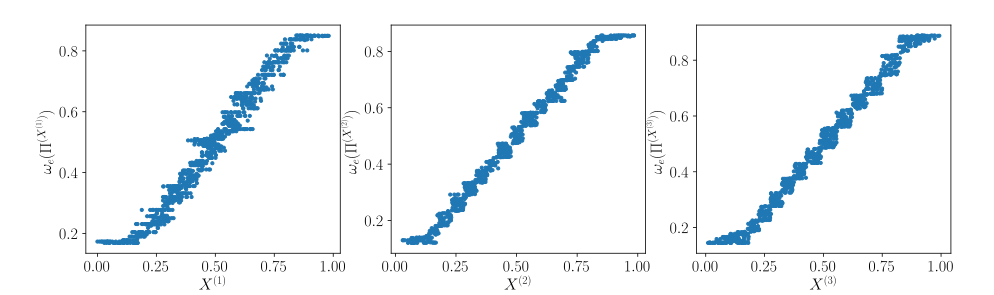
\includegraphics[width=\textwidth]{plan/zclosed-1-19999_error-P2}	
	\caption{Erreur de prédiction de $\inpx\m{1}$ dans le cas du plan pivoté en 3D. La prédiction est plus large car $U$ est quantifié plus grossièrement que dans le cas du cercle, voir figure~\ref{fig:2som_p_d}, mais elle est bien réalisée sur toutes les entrées. \label{fig:plan3_pred}}
\end{figure}

La disposition en étages qui apparaît sur les tracés d'erreur de prédiction vient directement de la disposition en zones des cartes de l'architecture. On peut donc supposer que la relaxation permet de choisir une zone; et la valeur prédite est prise au milieu de cette zone, d'où les \og étages \fg{} dans les tracés de prédiction.
Afin de valider l'influence des zones dans la capacité de prédiction d'entrée, voyons donc ce qui se passe dans le cas où les cartes ne se sont pas organisés en zones.
Pour cela, nous effectuons une phase d'apprentissage et prédiction sur une architecture dans laquelle $r_c = r_e$. 
Nous avions en effet vu que ce choix de paramètres n'engendre pas la formation de zones. L'erreur de prédiction qui en résulte est tracée en figure $\ref{fig:rcre_pred}$.
Nous observons que dans cette configuration, l'architecture de cartes n'est pas capable de réaliser la prédiction d'entrée manquante.
Nous ne pouvons cependant pas parler d'un apprentissage du modèle dans ca cas, car les cartes ne sont pas capable d'utiliser les relations entre entrées.
Les zones permettent donc bien aux cartes d'encoder les relations entre entrées et de les réutiliser en sortie et sont caractéristiques de l'apprentissage du modèle.

\begin{figure}
	\centering\includegraphics[width=0.9\textwidth]{rceqre/prediction.pdf}
	\caption{Prédiction de l'entrée $X\m{1}$ lorsque $r_c = r_e$. La prédiction n'est pas effectuée. Ainsi, sans formation de zones, la capacité de prise de décision n'est plus réalisable par une carte de l'architecture. \label{fig:rcre_pred}}
\end{figure}


\section{Influence des connexions sur l'apprentissage du modèle d'entrée}

Dans toutes les expériences précédentes, nous avons utilisé une architecture de cartes toutes connectées. 
Nous présentons maintenant quelques observations ouvrant des questions sur l'influence des connexions dans une architecture.
Nous étudierons d'abord un exemple d'architecture dans laquelle chaque carte possède un grand nombre de connexions. 
Nous nous intéresserons ensuite au cas d'une architecture de trois cartes dans laquelle chaque carte est liée à une seule autre et non aux deux autres.

\subsection{Influence d'un grand nombre d'entrées contextuelles sur l'organisation d'une carte}

Nous avons vu qu'une architecture de deux cartes apprenant sur le patch $[0,1]^2$ se déplie de manière à former deux échelles d'indices. Nous voulons étendre cette expérience pour des entrées de plus grande dimension et une architecture de plus de cartes. Nous pouvons donc effectuer la même expérience, mais our une architecture de $9$ cartes apprenant sur tout l'espace $[0,1]^9$, toutes connectées.
Nous nous demandons si les poids contextuels continuent de s'organiser en zones ou si le nombre de connexions modifie ce comportement. Nous tirons donc des entrées dans l'hypercube $[0,1]^9$. 
Nous ajoutons à ces entrées indépendantes une entrée $\inpx\m{10}$ identique à l'entrée $\inpx\m{9}$. 
Nous vérifierons sur les cartes $M\m{9}$ et $M\m{10}$ si la relation entre ces deux entrées est bien encodée par l'architecture ou si les connexions \og inutiles \fg{} de $M\m{9}$, c'est-à-dire correspondant à des modalités qui n'ont pas de dépendances avec $\inpx\m{9}$, viennent empêcher l'apprentissage de cette relation.

La figure \ref{fig:bigdim} présente la forme des poids de l'architecture de 10 cartes. Nous n'y avons pas représenté les entrées pour des raisons de lisibilité.
Nous remarquons que les poids contextuels tendent tous vers une valeur moyenne de 0.5 dans chaque carte pour les connexions relatives à des entrées indépendantes.
L'architecture équivaut donc à 9 cartes indépendantes, ce qui est logique par rapport à la disposition des entrées. Par contre, les couches poids contextuels correspondant aux entrées identiques dans $M\m{9}$ et $M\m{10}$ se déplient totalement, comme nous l'avions observé en figure~\ref{fig:id_results}.

De plus, la prédiction de l'entrée $\inpx\m{9}$ est bien réalisée lorsque la carte $M\m{9}$ ne reçoit pas cette entrée. Ainsi, il semble que les connexions relatives à des entrées indépendantes ont peu d'influence dans le calcul de l'activité par rapport aux connexions relatives à des entrées dépendantes.
Cette expérience mérite d'être étudiée plus en détail pour plus de types de dépendances entre entrées. 
En particulier, on peut se demander si ce comportement de l'architecture sur des entrées en grande dimension permet d'extraire automatiquement des relations entre entrées. Cette détection de relations serait également un comportement émergeant d'une architecture de cartes.

\begin{figure}[h!]
	\begin{minipage}{\textwidth}
	\includegraphics[width=\textwidth]{bigdim/weights.pdf}
	\end{minipage}
\begin{minipage}{\textwidth}
	\centering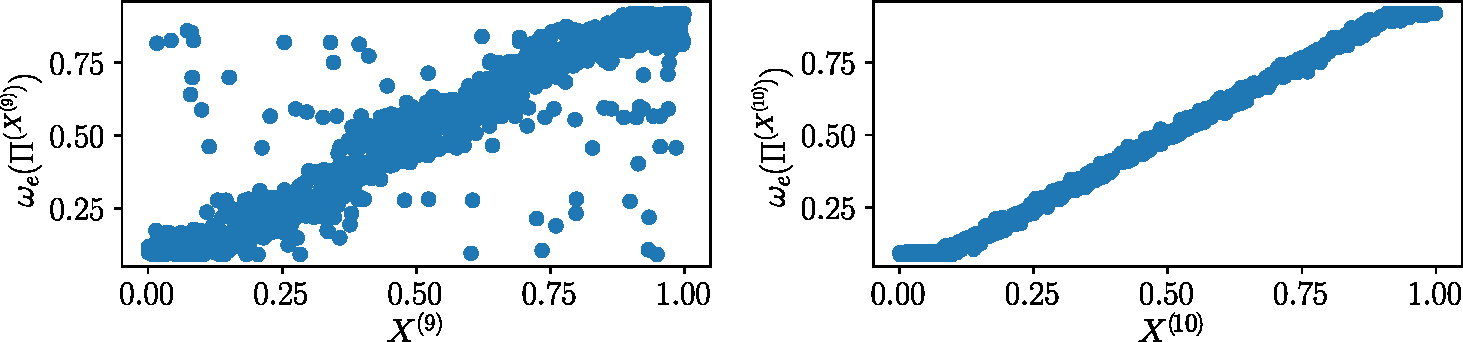
\includegraphics[width=0.8\textwidth]{bigdim/error_closed.pdf}
	\caption{En haut, tracé des poids des cartes pour une architecture de 10 cartes toutes connectées. Nous avons ici seulement tracé 4 cartes sur les 10. Les entrées sont indépendantes, sauf les entrées $\inpx\m{9}$ et $\inpx\m{10}$ qui sont identiques. Nous remarquons que les poids contextuels se moyennent autour de 0.5, sauf ceux correspondant aux entrées dépendantes. En pas, nous traçons l'erreur de prédiction de la carte 9 lorsqu'elle ne reçoit pas d'entrée. La prédiction est bien réalisée~: les connexions contextuelles inutiles ne polluent pas l'apprentissage. \label{fig:bigdim}}
\end{minipage}
\end{figure}

\subsection{Influence des connexions distantes sur l'organisation d'une carte}

A contrario d'un grand nombre de connexions, nous cherchons à observer comment une carte d'une architecture influence une carte distante, c'est-à-dire une carte qui ne lui est pas directement connectée.
Dans cette deuxième expérience, nous repassons sur une architecture de trois cartes 1D et reprenons comme modèle entrée le cercle tourné en trois dimensions (\textbf{G)}. 
Nous comparons le comportement de l'architecture dans laquelle les cartes sont connectées réciproquement, présentée plus haut, à celui d'une architecture de trois cartes en boucle, dans laquelle chaque carte est uniquement connectée à une seule autre carte. Ce modèle d'architecture est illustré en figure~\ref{fig:archi_loop}~: $M\m{1}$ est connectées à $M\m{2}$, $M\m{2}$ connectée à $M\m{3}$ et $M\m{3}$ connectée à $M\m{1}$.
En particulier, nous observerons si l'architecture est toujours capable de prédire $\inpx\m{1}$. Dans ce cas, la carte prédictive $M\m{1}$ ne reçoit en entrée que la position du BMU de $M\m{3}$~: la position du BMU de $M\m{2}$ intervient de façon distante dans le calcul de l'activité de $M\m{1}$. 

\begin{figure}[h!]
	\centering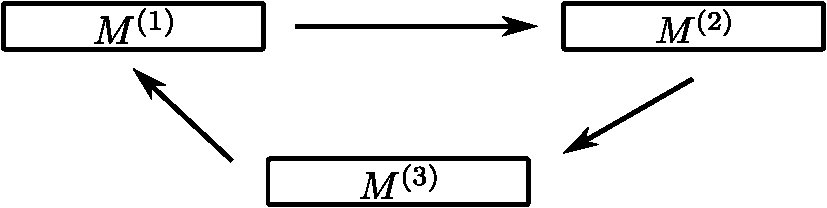
\includegraphics[width=0.5\textwidth]{loop/archi.pdf}
	\caption{Connexions dans une architecture en \og boucle\fg{}. \label{fig:archi_loop}}
\end{figure}

La disposition des poids et la capacité de prédiction sont tracées en figure~\ref{fig:3som_loop}.
L'architecture présente une organisation similaire au cas où les connexions sont réciproques~: Les poids contextuels forment des zones et $U$ est bien une fonction de $\bmu$ dans chaque carte. 
D'après la méthode d'étude présentée plus haut, nous pourrions dire que l'architecture a encodé le modèle d'entrées.
Cependant, la prédiction est moins bien réalisée que dans l'architecture avec rétroaction. 
Une partie des points est correctement prédite~: environ un tiers de points sont bien situé la diagonale du premier tracé.
Par contre, la prédiction échoue sur le reste des entrées. 

%conclusion ?

L'influence de ces connexions distantes est ainsi une piste d'étude pour un passage sur une grande architecture, dans laquelle nous pouvons agir sur les connexions entre cartes.


\begin{figure}[h!]
	\begin{minipage}{\textwidth}
		\centering\includegraphics[width=\textwidth]{loop/weights.pdf}
	\end{minipage}
	\begin{minipage}{\textwidth}
		\centering\includegraphics[width=\textwidth]{loop/prediction.pdf}
		\caption{Poids à l'issue de l'apprentissage et erreur de prédiction de $\inpx\m{1}$ dans une architecture de 3 cartes connectées en boucle. Bien que les poids s'organisent de façon similaire aux expériences dans lesquelles les cartes sont connectées réciproquement, la prédiction est moins bien réalisée. L'influence des connexions diminue donc rapidement avec la distance dans l'architecture, mais reste présente.\label{fig:3som_loop}}
	\end{minipage}
\end{figure}



\section{Application de la prédiction d'entrée à la commande d'un drone}

\subsection{Introduction}

Nous avons observé qu'après apprentissage, une architecture de cartes est capable de générer une entrée manquante de façon autonome. Cette entrée est cohérente avec le modèle d'entrée~: il s'agit d'une prédiction.
Nous sortons du cadre des entrées simulées pour nous placer dans un cas de contrôle réel.
Nous disposons d'un drone contrôlé à distance par ordinateur. Ce drone possède une caméra frontale ainsi qu'un ensemble de capteurs internes. Chacun de ces capteurs peut être considéré comme une modalité d'un espace multimodal. La commande envoyée au drone à chaque instant peut également être considérée une modalité de l'environnement. Lorsque le drone suit une trajectoire donnée, la commande envoyée à chaque instant est alors dépendante des valeurs des capteurs.


\'A l'aide d'une architecture de cartes, nous pouvons ainsi apprendre les relations existant entre les capteurs et la commande, afin de pouvoir générer la commande à envoyer au drone à partir des valeurs des capteurs lors d'une phase de prédiction.
Nous effectuerons cette phase de prédiction en temps réel, pendant laquelle la commande prédite sera envoyée au drône à chaque instant.
Le but de cette expérience est de tester l'architecture de cartes sur des cas d'entrées réelles, donc bruitées, en se plaçant dans un cadre de contrôle en temps réel d'un drone.
Nous évaluerons grâce à cette expérience la robustesse de l'algorithme à des données bruitées et la capacité de CxSOM à réagir en temps réel malgré les étapes de relaxation.

\subsection{Méthode expérimentale}

Le drone utilisé pour l'expérience est un quadricoptère. Il possède une caméra frontale.
Nous le contrôlons à distance par un ordinateur.  Lors de cette expérience, le drone naviguera dans un couloir en ligne droite. L'objectif du contrôle est que le drone se déplace au centre du couloir, en ligne droite.


La figure \ref{fig:drone} présente les capteurs et commandes disponibles.
Le drone est commandé par la définition d'un angle de rotation autour de chaque axe. 
L'angle autour de l'axe $z$ $\w$ contrôle la vitesse de rotation angulaire du drône autour de cet axe (lacet)
L'angle autour de l'axe $y$ (tangage) contrôle la vitesse de rotation haut/bas. Enfin, l'angle autour de $x$, $\rho$, influence l'\emph{accélération} du drone selon $y$ (roulis). Dans cette expérience, nous contrôlerons uniquement l'angle de roulis $\rho$ à l'aide d'une architecture de cartes.
L'angle de lacet $\omega$ sera contrôlé à l'aide d'un PID de façon à ce que la caméra du drone reste fixée au milieu du couloir. L'angle de tangage $y$ est maintenu à 0 à l'aide d'un PID également, de façon à ce que le drone se déplace à une altitude constante.
La commande $\rho$ constitue une première modalité des entrées que nous allons considérer dans cette expérience.

Nous considérons trois éléments extraits des capteurs du drone et qui sont relatifs à sa position par rapport au couloir. Une analyse de l'image issue de la caméra frontale nous permet de récupérier l'abscisse du point de fuite du couloir $x$ et la différence entre les angles des lignes du couloir, notée $\varphi$.
Enfin, les capteurs internes du drone nous permettent de récupérer les vitesses linéaires $v_x,v_y,v_z$ à chaque instant selon chaque axe de déplacement. 
Comme nous contrôlerons l'angle $\rho$, donc une l'accélération linéaire selon $y$, nous nous intéresserons particulièrement à la vitesse linéaire en $y$ en tant que modalité.
Finalement, nous utiliserons quatre modalités lors du déplacement du drone~: l'abscisse du point de fuite $x$, l'angle duy couloir $\varphi$, la commande en angle de roulis $\rho$ et la vitesse linéaire courante en $y$ $v_y$.


Nous construisons une architecture CxSOM sur ces quatre modalités, composée de quatre cartes 1D connectées chacune aux trois autres, tracée en figure~\ref{fig:archi_drone}. Chaque carte prend une des modalités comme entrée externe.
La phase d'apprentissage est réalisée sur des trajectoires du drone dans le couloir contrôlées par un humain.
Lors de cette phase, nous avons utilisé un système de contrôle PID pour assister la commande humaine. 
Cette phase d'apprentissage est réalisée hors ligne~: nous normalisons les entrées puis les présentons aléatoirement lors de la phase d'apprentissage.
Chaque carte est de taille $500$. Les paramètres sont $r_e = 0.2$ et $r_c = 0.02$.
L'apprentissage a été effectué sur 4890 points, obtenus sur des trajectoires effectuées dans le même couloir que les trajectoires de test. Nous avons présenté ces points une seule fois, ce qui suffit à un bon dépliement des cartes.


Après apprentissage, nous effectuons une phase de prédiction en ligne et en temps réel sur le contrôle du drone.
Lors de cette étape, la commande $\rho$ n'est pas présentée à la carte $M\m{\rho}$. $\w_e\m{\rho}(\bmu\m{\rho})$ et la valeur de la prédiction est utilisé comme commande $\rho$ envoyée au drône en temps réel.
Les angles de tangage et de lacet sont quant à eux contrôlés par un PID afin de maintenir l'axe du drone pointant vers le centre du couloir et une altitude constante.

\begin{figure}
	\centering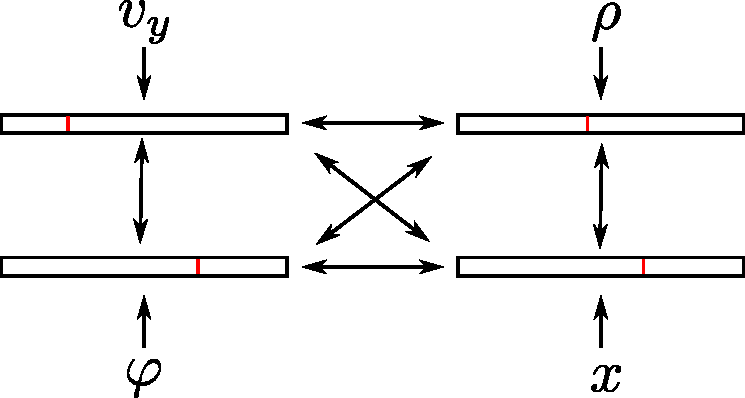
\includegraphics[width=0.5\textwidth]{archi_drone.pdf}
	\caption{Architecture de quatre cartes utilisée dans l'expérience. Chaque carte prend une modalité en entrée externe lors de l'apprentissage~: $v_y,\rho,\varphi,x$. Lors de la phase de prédiction, l'entrée $\rho$ n'est plus présentée à l'architecture et la commande envoyée au drône est $\w_e\m{\rho}(\bmu\m{\rho})$\label{fig:archi_drone}}.
\end{figure}

Afin de visualiser les conditions de l'expérience, nous avons tracé les dépendances entre chaque modalité en figure~\ref{fig:drone_inp}.
Nous nous intéressons ici aux dépendances entre la commande $\rho$ qui est celle que nous prédirons et des autres modalités.
On remarque que $\rho$ dépend linéairement de l'angle du couloir $\varphi$, mais que cette dépendance est très bruitée. Elle dépend également de la vitesse interne du drone $v_y$. Par contre, les entrées correspondant à l'abscisse du point de fuite varient peu et la commande $\rho$ dépend peu de $x$.

\begin{figure}
	\begin{minipage}{0.5\textwidth}
	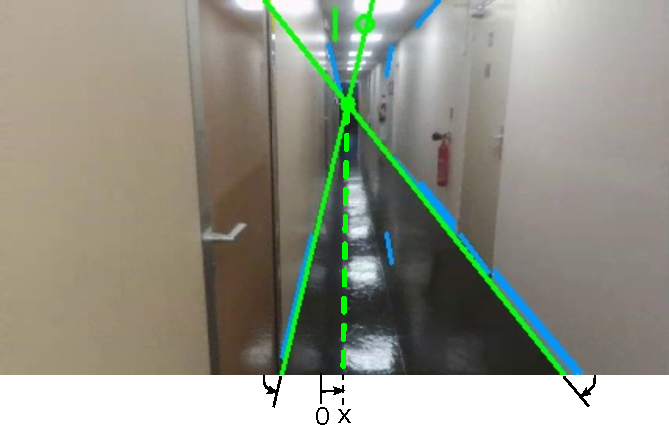
\includegraphics[width=\textwidth]{visudrone.pdf}
	\end{minipage}
	\begin{minipage}{0.5\textwidth}
	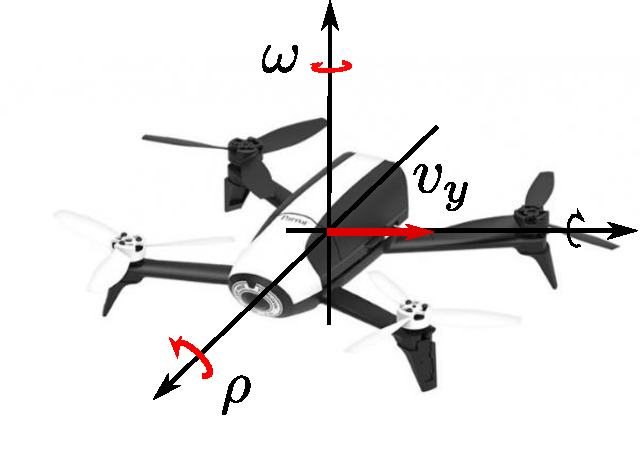
\includegraphics[width=\textwidth]{dronesteup}
	\end{minipage}
	\caption{Disposition des capteurs utilisés pour l'expérience}
	\label{fig:drone}
	\end{figure}

\begin{figure}
	\centering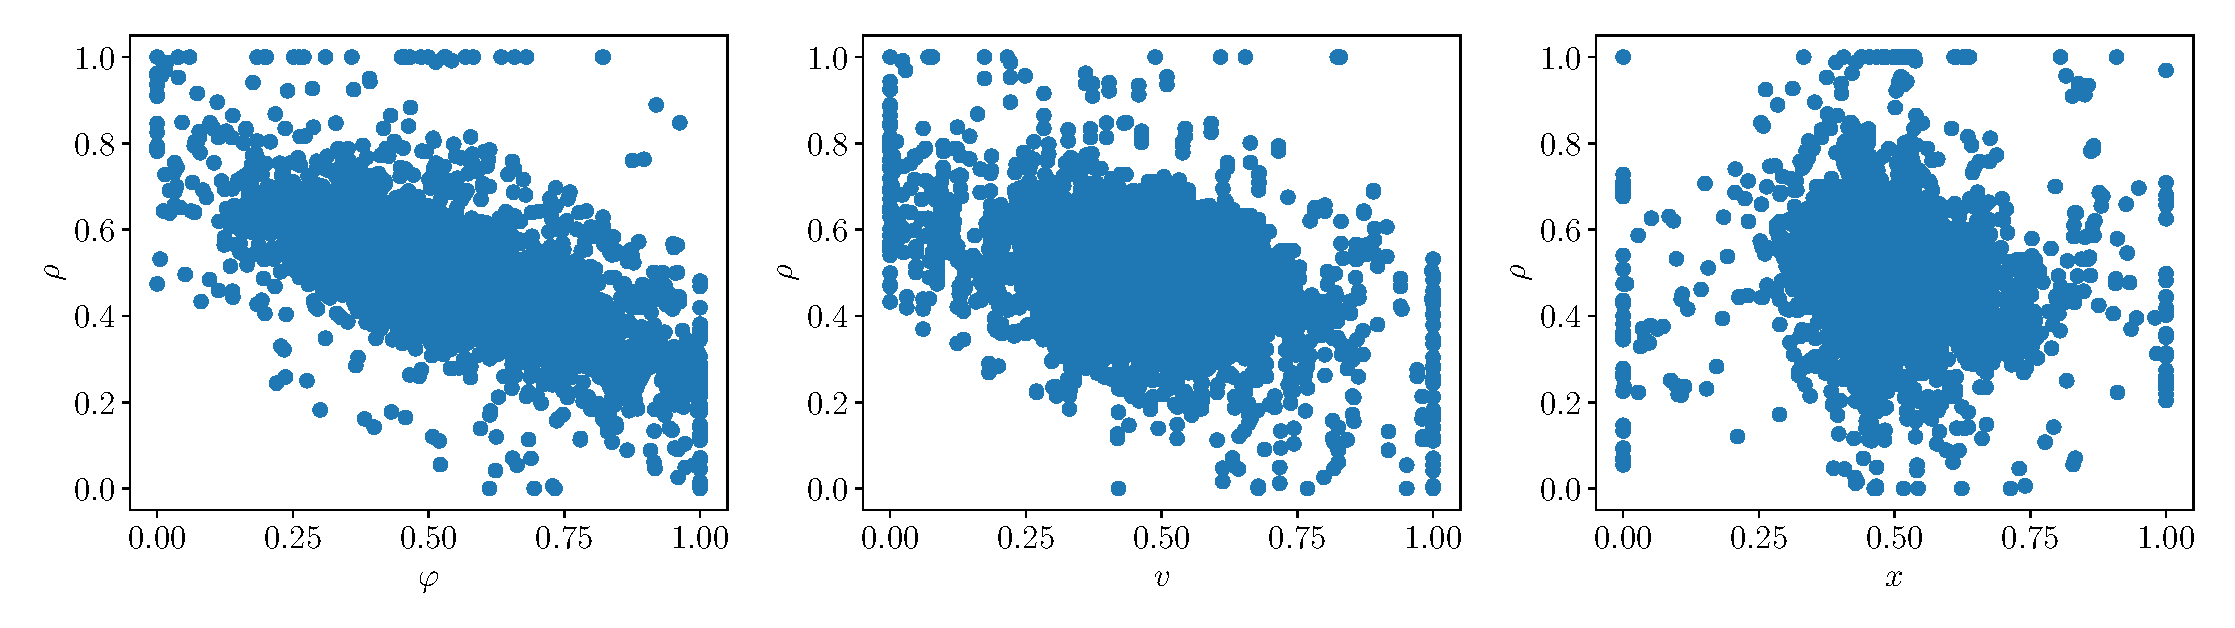
\includegraphics[width=\textwidth]{drone_inputs}
	\caption{Disposition et dépendances des entrées d'apprentissage. Nous chercherons à prédire $\rho$~: cette valeur dépend bien des autres modalités $v$, $\varphi$ et $x$. La dépendance est très simple (linéaire) mais très bruitée. \label{fig:drone_inp}}
\end{figure}


\subsection{Résultats}

La carte associée à $\rho$ possède une couche de poids externe et trois couches de poids contextuels. 
Ces poids sont représentés en figure \ref{fig:drone_w}. 

Nous observons d'abord que l'organisation des poids contextuels rappelle celle observé dans les dispositions d'entrée jouet~: les poids contextuels définissent des zones. 
La figure~\ref{fig:drone_w} présente en violet un exemple de calcul d'activité de la carte $\rho$. Cette activité est celle obtenue à l'issue de la relaxation. Il s'agit de l'activité globale de la carte prédictive.
Le BMU correspond au maximum de l'activité, ici $\bmu\m{\rho} = 0.41$.
Cela correspond à une valeur de prédiction $\w_e(\bmu\m{\rho}) = 0.49$. 
Lors de la phase de prédiction, cette valeur est remise à l'échelle et est la commande envoyée au drone.

Lors des expériences que nous avons effectuées, le drone apparaît voler correctement dans le couloir sans toucher les murs. Nous observons cependant que cette trajectoire est assez imprécise~: la commande prédite permet au drone de ne pas toucher les murs, mais ne lui permet pas de se centrer finement au centre du couloir.
La prédiction est donc correctement réalisée, toutefois assez imprécise. 
Cependant, le fait que les entrées soient très bruitées peut aussi expliquer le manque de précision. 


Cette capacité de prédiction montre une possibilité d'application des architectures de cartes sur des données réelles. Nous avons utilisé ici une architecture de quatre cartes, contrairement aux parties précédentes ou nous avons seulement utilisé des architectures de deux et trois cartes. 
Les résultats des expériences montrent ainsi que les comportements des architectures de deux et trois cartes sont toujours observés sur 4 cartes.
Malgré les données bruitées, l'architecture de cartes détecte une relation entre entrée qui lui permet de prédire de façon large la commande à envoyer.
Enfin, la réactivité de l'envoi de la commande au drone montre que la relaxation permet une réponse en temps réel.
Ces observations sont sur un cas simple d'application en une dimension, mais laissent la porte ouverte à une application possible des architectures CxSOM en pratique, par exemple en robotique.

Du travail supplémentaire est cependant nécessaire pour une réelle application de l'architecture.
Tout d'abord, il serait intéressant d'étudier l'application sur des données moins bruitées et disponibles en simulation afin de mesurer l'erreur de prédiction relative à l'architecture, comme une étape intermédiaire entre les données géométriques et le cadre réel. 
Plus généralement, les entrées d'une application robotique sont en pratique en plus grande dimension, par exemple une représentation d'une image. Il sera nécessaire d'étudier l'organisation des cartes sur ce type de données, en utilisant dans ce cadre des cartes en deux dimensions.

\begin{figure}
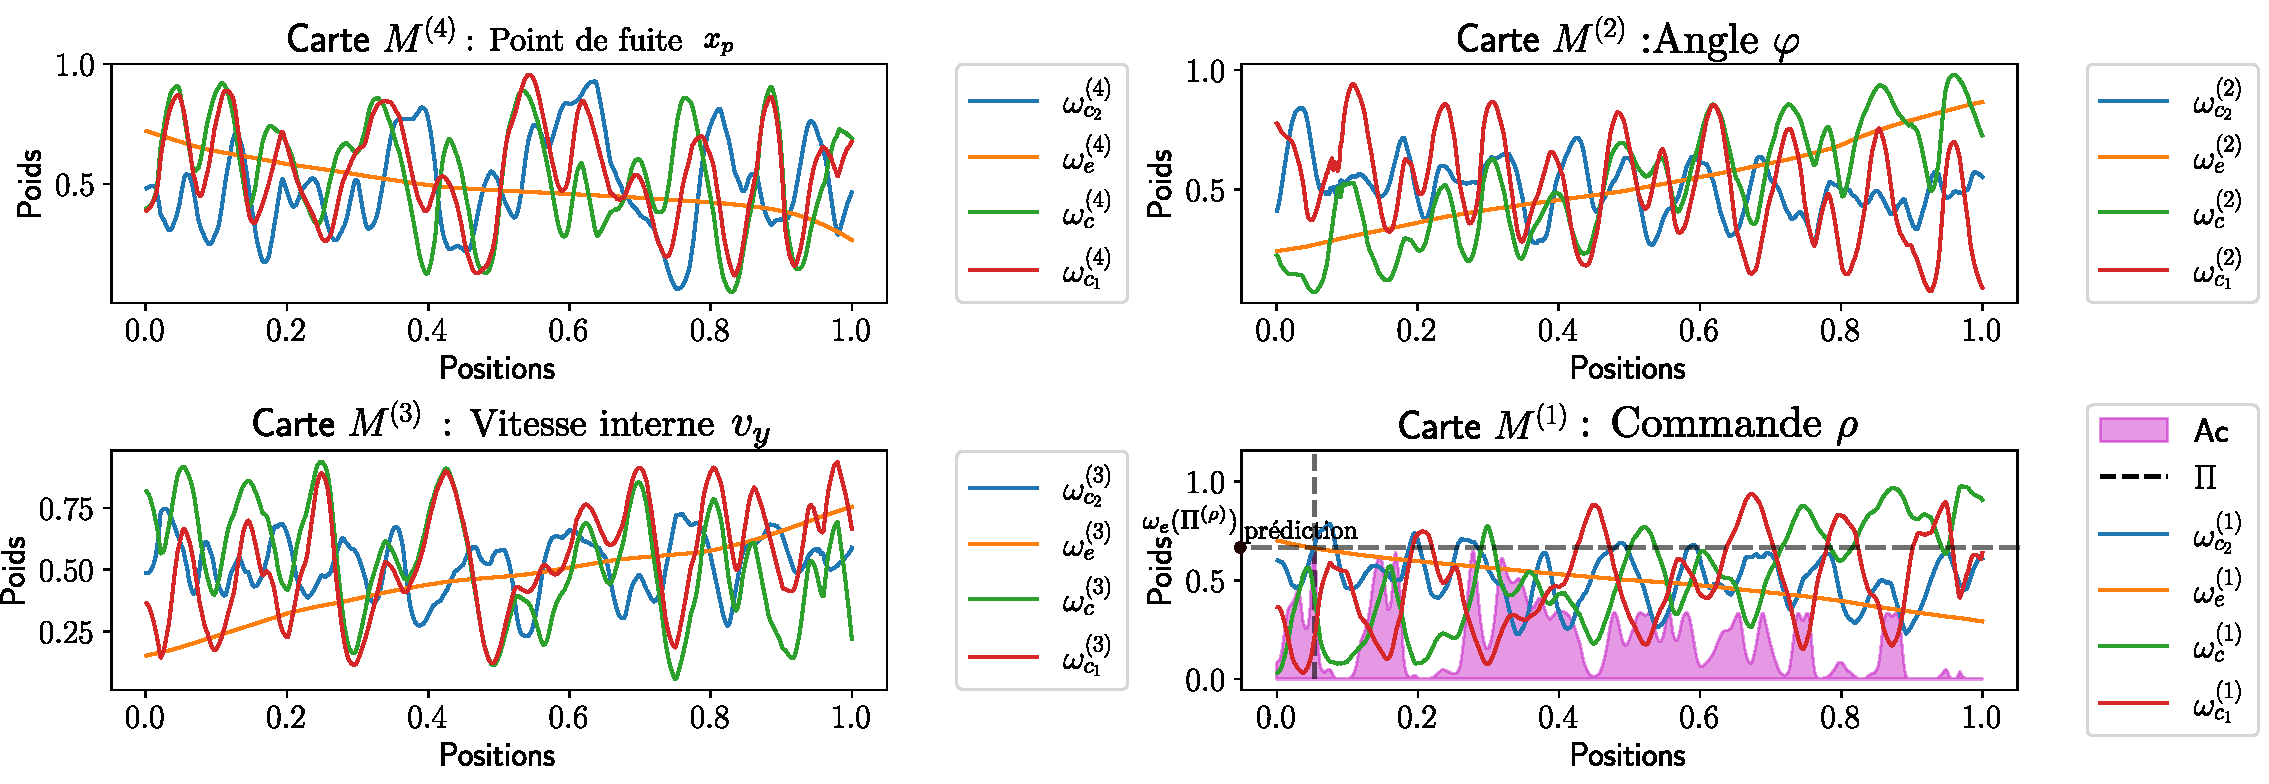
\includegraphics[width=\textwidth]{drone_weights.pdf}
\caption{Disposition des poids des 4 cartes après apprentissage.}
\label{fig:drone_w}
\end{figure}

\section{Conclusion}

Ce chapitre de résultats présente l'analyse de l'organisation d'architectures de 2 et 3 cartes 1D sur des données d'entrées en deux et trois dimensions.
Nous avons d'abord observé que l'apprentissage du modèle d'entrée dans une architecture CxSOM est marqué par une organisation à deux échelles~: les poids externes se déplient sur l'espace d'entrée comme les poids d'une carte classique. Les poids contextuels se déplient sur des sous-régions de la carte définies par la valeur de l'entrée externe, formant une disposition en \og zones \fg{}.
Ces zones de poids contextuels permettent d'encoder l'information sur tout le modèle d'entrée dans chacune des cartes~: 
chaque carte choisit ainsi son BMU en fonction à la fois de son entrée externe et de ses entrées contextuelles. Une position de BMU encode en une même valeur l'ensemble du modèle d'entrée et non seulement l'entrée externe de la carte.


Nous avons ensuite constaté que cette organisation en zones permet à l'architecture de générer des valeurs d'entrées qui correspondent au modèle appris.
Après apprentissage, une carte qui ne reçoit plus son entrée externe peut définir un BMU grâce à ses activités contextuelles et le poids externe du BMU est utilisé comme valeur générée de la modalité non présentée à la carte.
Dans ces tâches de prédiction, l'architecture CxSOM utilise de façon autonome le fait qu'elle ait encodé le modèle d'entrée. 
Nous avons observé que cette capacité de prédiction est directement liée à la présence des zones de poids contextuels, ce qui valide le fait que l'encodage du modèle vient bien de cette organisation en zones.
Cette capacité de prédiction est une application possible des architectures de cartes, mais permet également d'évaluer l'apprentissage d'un modèle d'entrée par l'architecture lorsque ce modèle n'est pas connu.


Maintenant que nous avons observé les comportements d'apprentissage dans des architectures de 2 et 3 cartes, une perspective principale d'étude de CxSOM est la construction d'architectures comportant plus de cartes.
Dans ces architectures, le choix des connexions entre cartes constitue un degré de liberté supplémentaire.
Pour mener à bien cette construction, une étude plus générale de l'influence des connexions permettra d'ajouter cette dimension à la conception de systèmes CxSOM.
Nous avons présenté dans ce chapitre deux perspectives d'influence des connexions entre les cartes.
D'une part, nous avons vu que des connexions distantes permettent toujours à l'architecture de cartes d'apprendre un modèle d'entrée. Cependant, lors de la prédiction, les cartes distantes de la carte prédictive ont moins d'influence que les cartes qui lui sont directement connectées. Cette observation montre que la connectivité d'une architecture est bien un paramètre ayant une grande influence sur l'apprentissage. 
Ensuite, nous avons observé qu'a contrario que la présence de nombreuses entrées contextuelles amène les poids contextuels à s'organiser vers une valeur moyenne des entrées. Dans le cas ou ces entrées sont indépendantes au sein du modèle d'entrée, ce comportement de moyennage permet aux activités contextuelles d'effacer leur contribution dans le calcul de l'activité globale~; cette dernière ne prendra alors en compte que les entrées qui ont une dépendance réelle.
Cependant, ce comportement de moyennage n'est pas souhaitable si les entrées ont toutes une relation entre elles, par exemple si $U$ est en grande dimension.


Une perspective d'étude nécessaire est ainsi d'évaluer la distribution de l'encodage du modèle d'entrée dans les cartes. 
Dans les expériences présentées dans ce chapitre, plus globalement dans cette thèse, le modèle $U$ est une variable 1D. 
Nous avons observé que l'apprentissage se traduit par le fait que $U$ est une fonction de $\bmu$ dans chaque carte.
Dans une grande architecture apprenant sur des entrées multimodales de dimension totale supérieure, on ne peut pas attendre que chaque carte encode la totalité du modèle $U$~: le nombre de n\oe{}uds est limité et l'architecture se contenterait d'apprendre la valeur moyenne de $U$, comme dans l'architecture de 10 cartes de ce chapitre.
On voudrait donc que $U$ ait une représentation distribuée au travers des cartes de l'architecture. 
Cette distribution de la représentation de $U$ n'apparaît pas clairement dans les expériences sur deux et trois cartes car les architectures sont trop petites pour pouvoir étudier cette propriété.
Cet aspect distribué de l'apprentissage est un point à étudier sur des architectures de plus grande taille, et si besoin à corriger en adaptant les paramètres du modèle pour envisager un développement du modèle CxSOM à grande échelle. 
Il sera par exemple possible de jouer sur les connexions, les paramètres des cartes ou le calcul d'activité.

Enfin, toutes ces expériences ont été menées sur des cartes 1D apprenant à représenter des données en une dimension. Ce cas de figure est rarement rencontré en pratique et il serait intéressant d'évaluer l'apprentissage sur des dimensions d'entrées supérieures. Pour une tâche de quantification vectorielle classique par une SOM, il est plus usuel d'utiliser des cartes en deux dimensions qui forment un bon compromis entre la capacité de quantification vectorielle rendue possible et le coût des calculs pendant l'apprentissage. Nous chercherons donc à utiliser des cartes 2D dans une architecture CxSOM. Le passage de 1D à 2D n'est pas immédiat et pose de nombreuses questions quant à l'organisation des poids et la recherche de BMU par relaxation. Nous présenterons à ce propos au chapitre \ref{chap:analyse2D} des expériences préliminaires étudiant l'organisation des poids dans une architecture de cartes en deux dimensions.

\ifSubfilesClassLoaded{
    \printbibliography
    %\externaldocument{../main.tex}   
}{}
\end{document}


% Nous prendrons ensuite deux configurations d'entrées en trois dimensions, tracées en figure~\ref{fig:inputs_3D} pour les architectures de trois cartes~:
% \begin{itemize}
% 	\item Les entrées sont sur un cercle en 2D, pivoté sur les trois dimensions. $U$ est une variable 1D. (Entrées \textbf{G})
% 	\item Les entrées sont dans un plan 2D pivoté sur les trois dimensions. $U$ est une variable 2D. (Entrées \textbf{H})
% \end{itemize}

% Dans ces deux cas, la connaissance de deux des entrées ainsi que du modèle détermine la valeur de la troisième entrée. 
% Nous étudierons ces configurations dans un cadre de prédiction d'entrées~: nous donnons en entrées $X\m{1}, X\m{2}$ à la structure et regardons si la valeur de $X\m{3}$ correspondante est correctement prédite par l'architecture. 
% Une bonne prédiction témoigne de l'apprentissage du modèle d'entrées par l'architecture de cartes.
% Les architectures de cartes deux dimensions seront traitées au chapitre~\ref{chap:analyse2D}.

% \subsubsection{Matériel}
% Le code utilisé pour générer les expériences et les représentations est disponible en ligne \footnote{\url{todo.github.com}}
% Il s'appuie sur la librairie CxSOM \footnote{\url{https://github.com/HerveFrezza-Buet/cxsom}}, développée au sein de notre équipe.
% Cette librairie permet d'implémenter des cartes de Kohonen simples ainsi que des architectures CxSOM spécifiquement.
% Cette librairie s'interface avec un module python (\emph{pycxsom}) afin de faciliter les représentations et manipulation des cartes pendant et après l'apprentissage.
% CxSOM permet de paralléliser au maximum les opérations indépendantes. Par exemple, la phase d'apprentissage des cartes est séquentielle car le calcul des valeurs des poids pour l'itération $i$ dépend de $i-1$, mais toutes les opérations de tests dans lesquelles le temps n'intervient pas s'exécutent en parallèle.
% Notons que la gestion du consensus lors de la relaxation passe également par des mécanismes locaux aux cartes dans notre implémentation. 
% Nous devons en effet vérifier lors de chaque pas de relaxation si les cartes ont atteint un consensus. Pour cela, chaque carte envoie un signal supplémentaire aux cartes voisines indiquant si son BMU a été modifié. Lorsque qu'une carte reçoit de toutes ses voisines que leur BMU n'est plus modifié et que le BMU de la carte n'a pas non plus été modifié lors de l'étape, la relaxation s'arrête dans cette carte.
% Les codes C++ et python que nous avons utilisé pour générer les expériences présentées dans ce chapitre sont disponibles sur git : REF.
% Le développement de la librairie CxSOM a été effectué en parallèle de cette thèse au sein de l'équipe. 
% Toutes les expériences présentées ici tournent sur un processeur i7 4 c\oe{}urs.